\section{Einführung}
Das folgende Pflichtenheft beschreibt die Anforderungen und Spezifikationen für die Entwicklung einer
Carsharinganwendung im Auftrag des Unternehmens Car Gateway (im Folgenden Auftraggeber bzw.\ der Kunde, Sie, Ihr oder Ihren genannt).
Als Ihr Auftragnehmer, die flojc.\ AG verpflichten wir uns, die notwendigen Funktionalitäten sowie technischen Anforderungen umzusetzen.

\subsection{Umfeld}
\label{subsec:1_1_umfeld}
Im Auftrag einer mittelständischen Autovermietung soll ein Softwaresystem entwickelt werden,
das eine automatische Abwicklung von Reservierungen, Fahrzeugverwaltung, Mitglieder- und Abrechnungsverwaltung
für den Einstieg in das Carsharing-Geschäft ermöglicht.
Dieses Dokument dient als Pflichtenheft und bildet die vertragliche Grundlage für das Projekt.
Es enthält die Anforderungen an das Softwaresystem aus Auftragnehmer-Sicht, welche nach Bestätigung durch den
Kunden in konkrete technische Spezifikationen umgesetzt werden.
Zusätzlich werden interne und externe Subsystem- und Systemschnittstellen in separaten Schnittstellendokumenten definiert.
Die technischen Spezifikationen dienen später als Grundlage für den Entwurf der Systemarchitektur und der Subsysteme.
Es ist von besonderer Bedeutung, den Kunden durch eine sorgfältige Arbeit und ein zufriedenstellendes Endprodukt für
weitere Aufträge zu gewinnen, da keine vorherige Kundenbeziehung besteht.

\subsection{Ausgangssituation und Ziele}
Die flojc.\ AG ist seit über 10 Jahren auf die Entwicklung, den Vertrieb und die Administration von Software-Kommunikationssystemen spezialisiert.
Sie haben uns beauftragt, das in \autoref{subsec:1_1_umfeld} genannte Softwaresystem zu entwickeln.
Ziel des Systems ist es, Ihnen den Einstieg in das Carsharinggeschäft zu ermöglichen, Arbeitsabläufe zu digitalisieren und wiederkehrende Prozesse zu automatisieren, um die Mitarbeiter zu entlasten und Kosten zu sparen.
Durch die Digitalisierung soll zudem eine höhere Erreichbarkeit für Ihre Kunden erzielt werden.


\subsection{Umfang und Art des vorgeschlagenen Systems}
Das System besteht aus einem Softwaresystem und der dazugehörigen Hardware,
einschließlich der Dokumentation.
Grundlegend soll das System eine automatische Abwicklung der Buchungen,
Verwaltung der Fahrzeuge, Mitglieder und Abrechnungen ermöglichen.
Es ist darauf ausgelegt, eine hohe Erreichbarkeit zu gewährleisten.
Dafür bietet es Ihren Kunden verschiedene Möglichkeiten, ein Mitgliedskonto anzulegen oder zu verwalten:
entweder direkt in der Filiale, telefonisch oder online. \medskip

Darüber hinaus verfügt das System über eine benutzerfreundliche Web-Schnittstelle,
welche für alle Nutzer den Zugang ermöglicht.
Innerhalb der Web-Schnittstelle kann sich der Nutzer anmelden,
sofern er bereits über ein Konto verfügt.
Sobald die Anmeldung durchgeführt wurde, wird der Gast als Mitglied, Mitarbeiter oder Admin
klassifiziert und erhält die ihm zustehenden Rechte und Funktionalitäten.
Darüber wird beispielsweise den Mitarbeitern ermöglicht, den Fahrzeugpool, die Ausleihstationen und die
Abrechnungen zu verwalten.
Somit ist der einzige Berührungspunkt aller Nutzer mit dem System die Web-Schnittstelle.
Dabei wird ein besonderes Augenmerk auf den Schutz der Kunden- und Firmendaten gelegt,
indem alle übermittelten Daten verschlüsselt werden. \medskip

Um Ihren Kunden ein bestmögliches Nutzungserlebnis zu bieten, benötigt das System weitere Schnittstellen.
Eine solche Schnittstelle ermöglicht es beispielsweise Ihren Kunden,
reservierte Fahrzeuge mithilfe einer RFID-Karte oder eines vergleichbaren Systems zu nutzen. \medskip

Ein besonderes Alleinstellungsmerkmal des Systems ist die Anbindung
an das bestehende Buchhaltungssystem Ihres Unternehmens.
Darüber hinaus soll das System ausfallsicher sein,
mehrere Sprachen unterstützten und idealerweise automatisierte Workflows vorweisen. \medskip

Da Sie davon ausgehen, dass es ca.\ 5000 Mitglieder, 25 Fahrzeuge und 5 Stationen pro Standort
bei einer Anzahl von 10 Standorten geben wird, muss bei der Entwicklung des Systems auf die Robustheit
sowie die Leistungs-/ Performanceanforderungen geachtet werden.
Das zu liefernde Softwaresystem besteht aus einem Frontend, Backend und einer Datenbank,
auf der u.a.\ Kundendaten gespeichert und verwaltet werden.
Die Hardware umfasst RFID-Karten, RFID-Lesegeräte und GPS-Tracker.
Die Dokumentation des Projekts enthält das Pflichtenheft, die technische Dokumentation,
das Product Backlog der Zwischenergebnisse und einen Projektplan.

\subsection{Abweichung: Pflichtenheft vs. Lastenheft}
Das Lastenheft definiert die Anforderungen an das System, während das Pflichtenheft beschreibt,
wie diese Anforderungen umgesetzt werden sollen.
Die Anforderungen wurden vorher aufgeteilt, um eine leichtere Rückverfolgbarkeit (traceability) zu erzielen.
Im Pflichtenheft wurden die Anforderung nach dem MoSCoW-Prinzip (muss, soll, kann) priorisiert, um die einzelnen Anforderungen
nach ihrer Relevanz im Gesamtsystem zu strukturieren und implementieren.
Weitere Unterschiede zwischen Lasten- und Pflichtenheft sind nicht aufgetreten.

\subsection{Definitionen, Akronyme und Abkürzungen}
\begin{table} [H]
    \centering
    \caption{Definitionen}
    \begin{tabularx}{\textwidth}{|l|X|}
        \toprule
        \textbf{Abkürzung} & \textbf{Bedeutung} \\
        \hline
        A & Verifikationsmethode: Analyse \\
        \hline
        DSGVO & Datenschutz-Grundverordnung\\
        \hline
        GPS & Global Positioning System \\
        \hline
        I & Verifikationsmethode: Inspektion\\
        \hline
        IDE & integrierte Entwicklungsumgebung \\
        \hline
        N/A & nicht Angegeben \\
        \hline
        PC & Personal Computer \\
        \hline
        RFID & Radio-frequency identification \\
        \hline
        RoD & Verifikationsmethode: Review of Design\\
        \hline
        T & Verifikationsmethode: Test\\
        \hline
        UC & UseCase \\
        \bottomrule
    \end{tabularx}\label{tab:Definitionen}
\end{table}

\begin{table} [H]
    \centering
    \caption{Akronyme}
    \begin{tabularx}{\textwidth}{|l|X|}
        \toprule
        \textbf{Akronym} & \textbf{Bedeutung} \\
        \hline
        Gast & Eine Person, welche noch nicht angemeldet ist.\\
        \hline
        Mitglied & Eine Person, welche mit ihrem Mitgliedskonto angemeldet ist.
        Verwalten des eigenen Kontos und Buchungen sind möglich. \\
        \hline
        Mitarbeiter & Eine Person, die sich als Mitarbeiter auf dem System angemeldet hat.
        Verwalten aller Konten, des Fahrzeugpools sowie der Belegung und aller Buchungen sind möglich \\
        \hline
        Admin & Eine Person, die sich als Admin angemeldet hat, verfügt über die Rechte des Mitarbeiters hinaus, die Fähigkeit ein Mitarbeiterkonto anzulegen und zu löschen    \\
        \bottomrule
    \end{tabularx}\label{tab:Akronyme}
\end{table}


\section{Bezug zu Dokumenten}

\subsection{Anwendbare Dokumente}
\begin{table} [H]
    \centering
    \caption{Anwendbare Dokumente}
    \begin{tabularx}{\textwidth}{|X|X|}
        \toprule
        \textbf{Name} & \textbf{Beschreibung}\\
        \hline
        Laborprojekt Carsharing System HS Bremen FK4 Softwaretechnik 2 Sommersemester 2023 Prof.\ Dr.\ -Ing.\ Jasminka Matevska & beinhaltet die Beschreibung des Laborprojektes, sowie die notwendigen Anforderungen. \\
        \hline
        Frequently Asked Questions - Laborprojekt CarSharing Softwaretechnik 2 SoSe 2020 Prof.\ Dr.\ -Ing.\ Jasminka Matevska & beinhaltet eine Sammlung mit weiteren, möglichen Anforderungen an das Projekt. \\
        \bottomrule
    \end{tabularx}\label{tab:Anwendbare Dokumente}
\end{table}

\subsection{Referenzierte Dokumente}
\begin{table} [H]
    \centering
    \caption{Referenzierte Dokumente}
    \begin{tabularx}{\textwidth}{|X|X|}
        \toprule
        \textbf{Name} & \textbf{Beschreibung} \\
        \hline
        Rahmenbedingungen für Carsharing- und
        Scootersharing-Unternehmen und die Ziele und Maßnahmen im
        Zusammenhang mit der Elektromobilitätsstrategie der
        Bundesregierung & Rahmenbedingungen zum CarSharing des Deutschen Bundestags. \\
        \hline
        Datenschutz-Grundverordnung (DSGVO) & Verordnung der Europäischen Union.\ Beinhaltet Regeln zur Verarbeitung personenbezogener Daten. \\
        \bottomrule
    \end{tabularx}\label{tab:Referenzierte Dokumente}
\end{table}


\section{Voraussetzungen}
\label{sec:vorraussetzungen}

\subsection{Hardware Umgebung}
\label{subsec:hardware_umgebung}
Um die Software zu verwenden, sollen die bereits vorhandenen Windows-PCs weiterhin verwendet werden.
Diese sind mindestens mit einem Intel Core i5 Prozessor der 5.\ Generation ausgestattet.
Zusätzlich besitzen sie einen Arbeitsspeicher von mindestens 8 GB und einen Festplattenspeicher von mindestens 500 GB
in Form einer HDD\@.
Als Grafikkarte wird eine standard Intel HD-Grafikkarte oder besser verwendet.
Des Weiteren sind bereits mehrere Linux-Server vorhanden, welche weiterhin verwendet werden können.
Sollte die Leistung dieser nicht ausreichen,
können wir die Server mit besseren Hardware-Komponenten ausstatten.

\subsection{Software Umgebung}
\label{subsec:software_umgebung}
Da im Unternehmen bereits mehrere Linux-Server vorhanden sind, sollte das Backend mit dem Linux-Betriebssystem
kompatibel sein.
Dies wird mit der Hilfe der Containervirtualisierungssoftware Docker realisiert.
Diese kann auf den Servern installiert werden.
Da auf den PCs des Unternehmens Windows installiert ist, sollte das Frontend, was von den Mitarbeitern bedient wird
mit Windows kompatibel sein.
Dies wird erreicht, indem diese Schnittstelle in Form einer Webanwendung zur Verfügung gestellt wird.
Ferner ist es geplant den Dienst auch als App anzubieten, die dieselben Funktionen beinhaltet.

\subsection{Entwicklungshilfsmittel}
\label{subsec:entwicklungshilfsmittel}
Vom Kunden wurden keine Entwicklungshilfsmittel vorgeschrieben.
Daher haben wir uns entschieden die IDE IntelliJ von JetBrains für die Entwicklung der Anwendung zu nutzen.
Des Weiteren wird für die Versionskontrolle Git verwendet.
Hierbei befindet sich das Repository auf Bitbucket, dabei handelt es sich um ein Produkt des Unternehmens Atlassian.
Das Product-Backlog wird ebenfalls mit einem Tool names Jira aus dem Hause Atlassian geführt.

\subsection{Verwendete Fremdprodukte}
\label{subsec:fremdprodukte}
Das Backend wird mit Java und Spring Boot entwickelt werden, da wir mit der
genannten Software bereits Erfahrung gesammelt haben und die beinhalteten Funktionen
die Entwicklung erleichtern.
Für die Entwicklung des Frontends haben wir uns für Flutter entschieden,
wobei es sich um ein UI-Entwicklungs-Kit von Google handelt.
Dieses ist zusätzlich Open-Source und es können Plattformunabhängige Apps, sowie Browseranwendungen in der
Programmiersprache Dart erstellt werden.
Nach der Registrierung soll eine Identitätsprüfung stattfinden.
Hierfür wird das Postident-Verfahren verwendet.
Des Weiteren soll eine Bonitätsprüfung stattfinden, was über eine SCHUFA Abfrage realisiert wird.
Die Abwicklung der Zahlungen wird von einem externen Dienstleister übernommen.
Dabei sollen die Zahlungen über Paypal, SEPA-Lastschrift, Kreditkarte und Überweisung möglich sein.


\section{Randbedingungen}

\subsection{Technische Randbedingungen}
Nach Absprache mit dem Kunden haben wir festgestellt, dass keine technischen Randbedingungen vorliegen.

\subsection{Terminliche Randbedingungen}
\label{subsec:terminliche_randbedingungen}
Als Auftragnehmer verpflichten wir uns folgende Termine einzuhalten:

\begin{table} [H]
    \centering
    \begin{tabular}{l|l}
        \toprule
        \textbf{Datum} & \textbf{Beschreibung}                                    \\
        13.07.2023     & Präsentation der Anwendung                               \\
        20.07.2023     & Übergabe der Anwendung                                   \\
        20.07.2023     & Abnahme und Tests                                        \\
        20.07.2023     & Übergabe der Dokumentationen (Anleitungen, Readme etc.)          \\
        24.07.2023     & Hands-on-Training: Einarbeitung der Mitarbeiter in die Anwendung  \\
        \bottomrule
    \end{tabular}
\end{table}

Um eine effektive Nutzung und maximale Leistungsfähigkeit der Anwendung sicherzustellen, ist eine gründliche Einarbeitung der zukünftigen Nutzer unerlässlich.
Zu diesem Zweck haben wir für den 24.07.2023 ein Hands-on-Training geplant, bei dem wir Ihren Mitarbeitern alle Funktionalitäten der Anwendung vorstellen werden.
Hierbei werden Ihre Mitarbeiter auch selbst aktiv werden können, um ein tieferes Verständnis für die Anwendung zu erlangen.

\subsection{Implementierungs- und Entwicklungsvorschriften}
Der Auftraggeber hat keine Implementierungs- oder Entwicklungsvorschriften aufgeführt.

\subsection{Rechtliche Randbedingungen}
Als Auftragnehmer liegt es in unserer Verantwortung, dass die Anwendung alle relevanten rechtlichen Randbedingungen einhält.
Dazu zählen: \medskip
\begin{itemize}
    \item Datenschutz: Die Verarbeitung personenbezogener Daten wie Name, Adresse oder Zahlungsinformationen durch die Anwendung entspricht den Datenschutzbestimmungen gemäß der Datenschutz-Grundverordnung (DSGVO).
    \item Haftung: Die Anwendung stellt die Haftungsregularien des Auftraggebers dar, die im Falle eines Unfalls oder Schadens gelten.
    \item Urheberrecht: Bei der Verwendung von Bildern oder Markennamen in der Anwendung wird sichergestellt, dass keine Urheberrechte verletzt werden.
    \item Verbraucherschutzrecht: Die Anwendung stellt sicher, dass die User angemessen über die Nutzungsbedingungen, die Preise und die Vertragsbedingungen des Auftraggebers informiert werden.
\end{itemize}

Der Bundestagsbeschluss zur Bevorrechtigung des Carsharings hat keine direkte Auswirkung auf die Carsharing-Anwendung.
Gemäß dem Beschluss soll das Konzept des Carsharing gefördert und unterstützt werden, indem bevorzugte Parkplätze oder Zufahrtswege für Carsharing-Fahrzeuge bereitgestellt werden.
Der Bundestagsbeschluss zur Bevorrechtigung des Carsharings hat keine direkte Auswirkung auf die Carsharing-Anwendung.

\subsection{Verpackungsanforderungen}
Die GPS-Tracker, RFID-Karten und -Leser sollen sicher verpackt sein, sodass diese beim Transport nicht beschädigt werden.

\subsection{Transportanforderungen}
Am Übergabetag, den 20.07.2023, soll die Anwendung auf einem Repository bereitgestellt werden.
Sämtliche Begleitdokumente sollen ebenfalls im PDF-Format auf dem Repository zu finden sein.
Die GPS-Tracker, RFID-Karten und -Leser sollen am Übergabetag an Sie ausliefert werden.

\subsection{Sonstige Randbedingungen}
Sonstige Randbedingungen sind nicht vorhanden.


\section{Funktionsumfang}

\subsection{Anwendungsfälle}

\subsubsection{Anwendungsfalldiagramm}
\begin{figure}[H]
    \label{fig:anwendungsfalldiagramm}
    \centering
    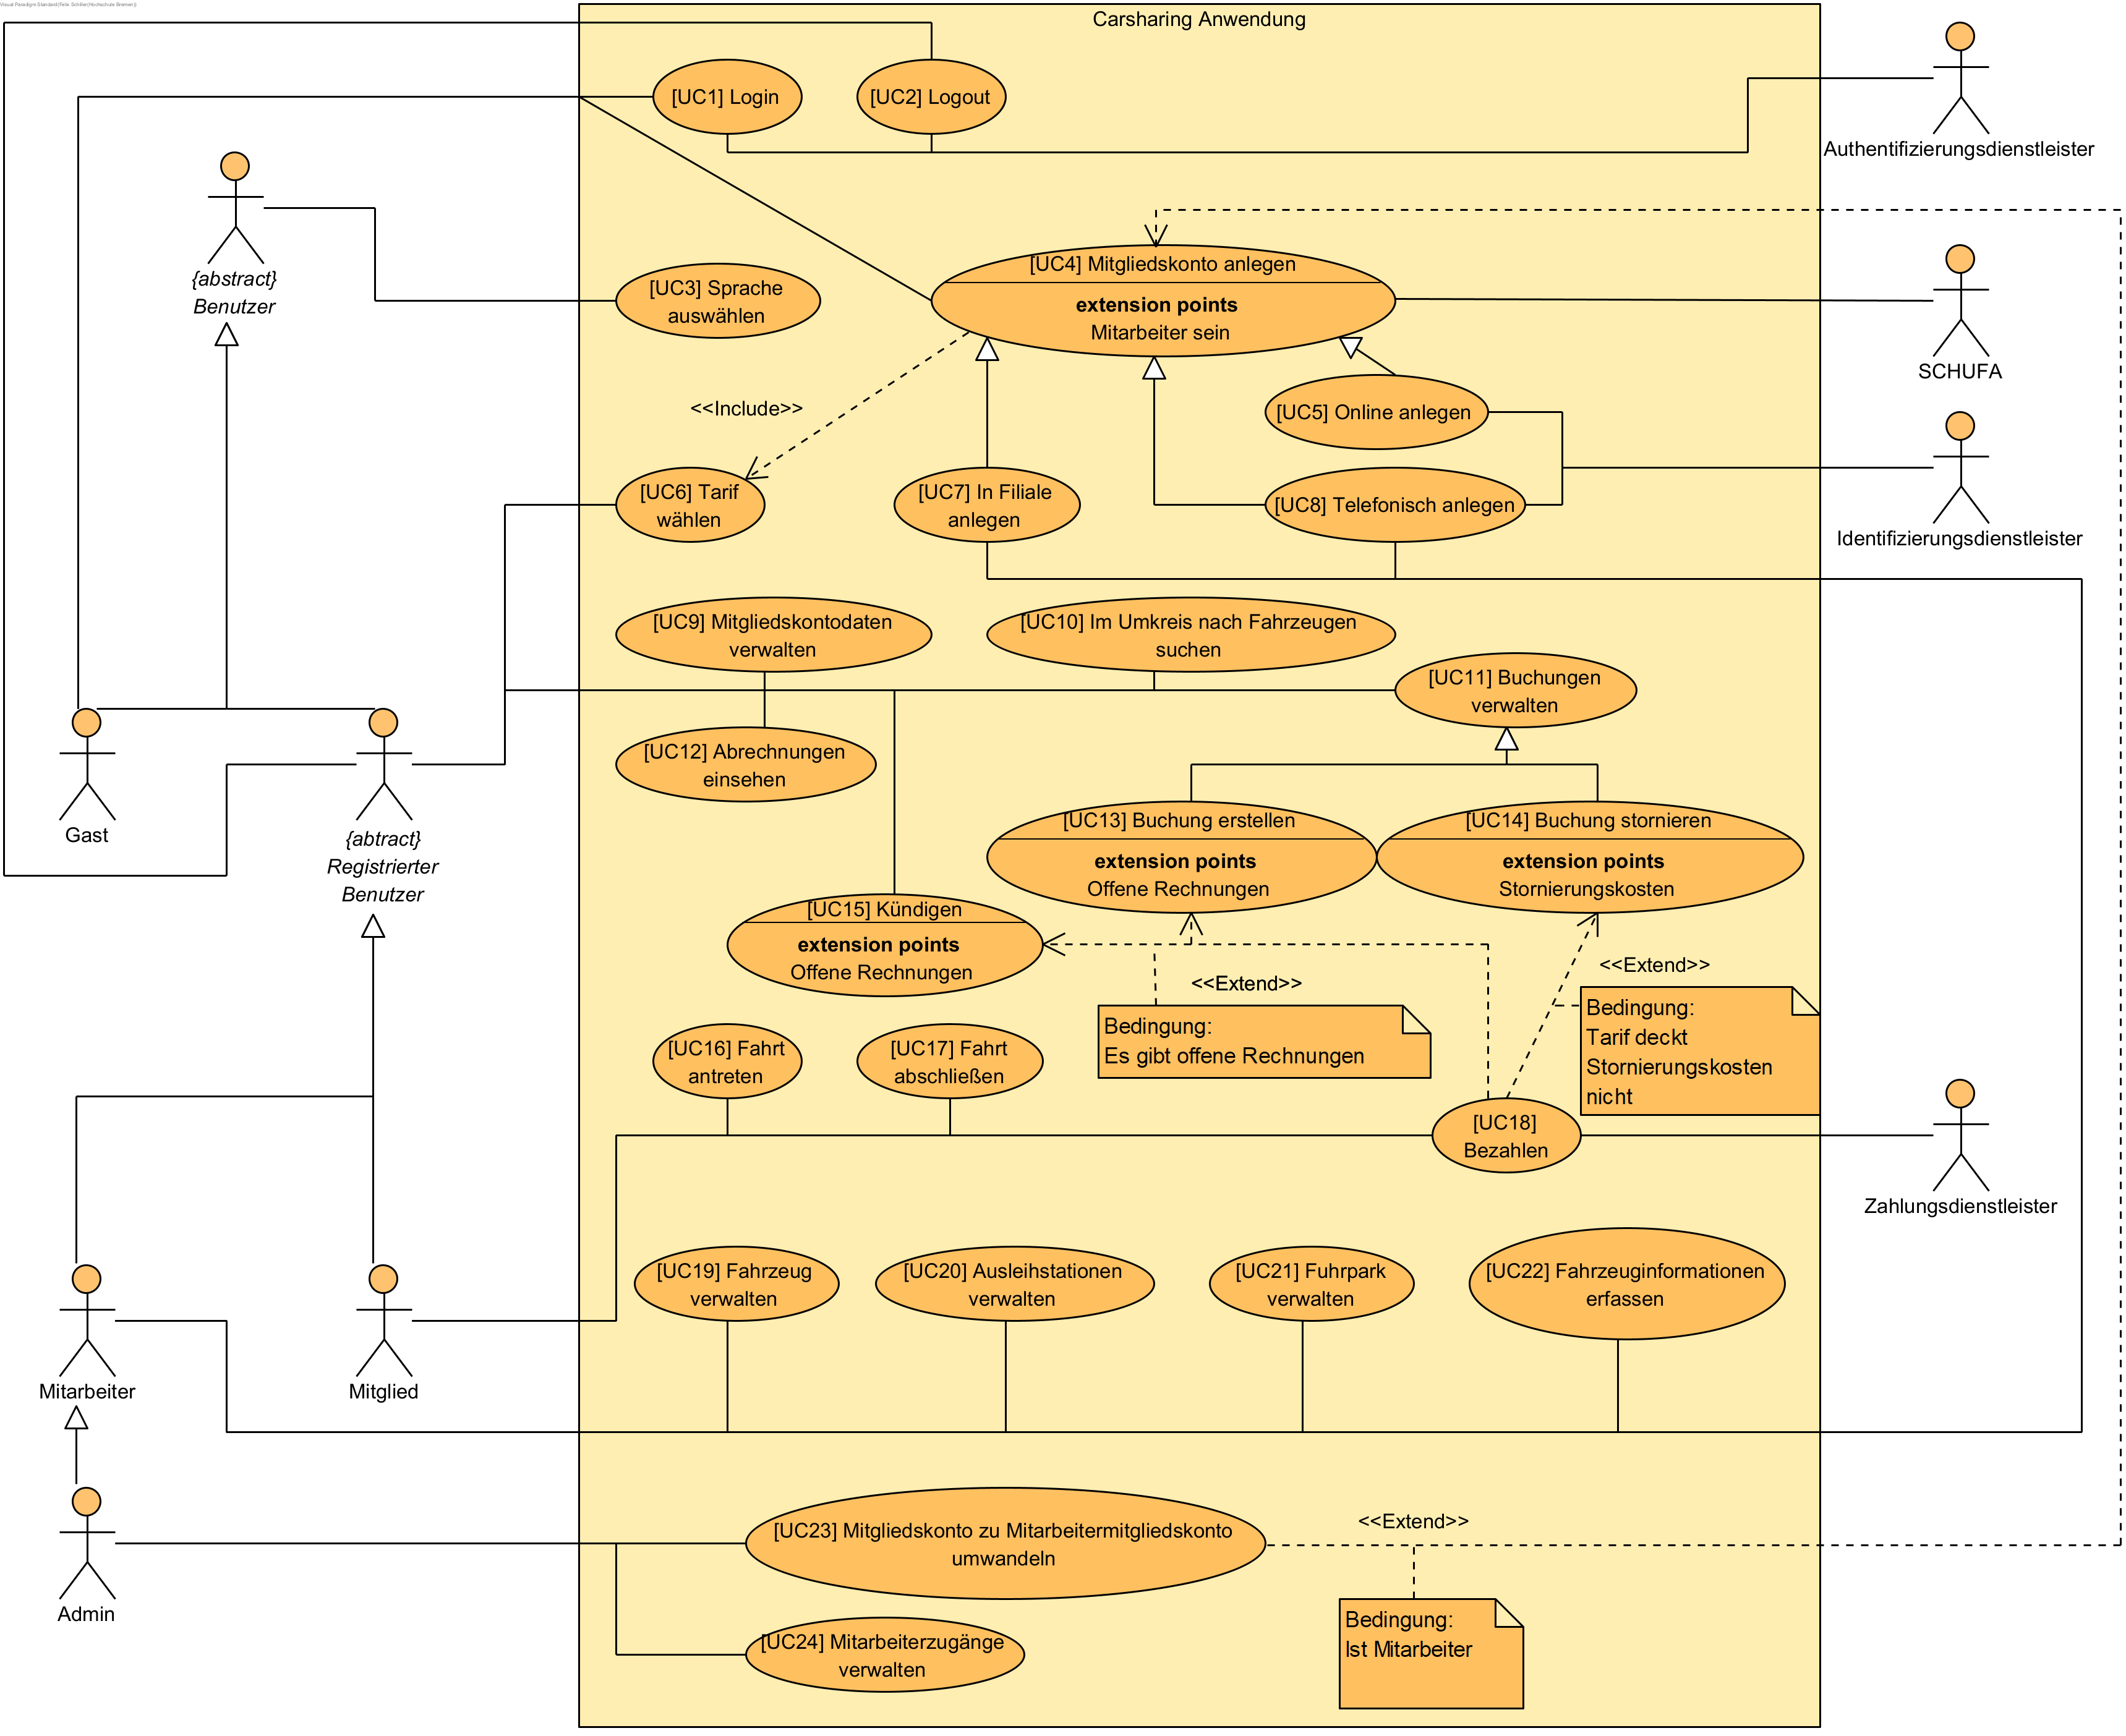
\includegraphics[width = \textwidth]{pictures/anwendungsfalldiagramm}
    \caption{Anwendungsfalldiagramm}
\end{figure}


\subsubsection{Beschreibung}
Das vorliegende Diagramm zeigt die Akteure und Anwendungsfälle, die wir aus den Anforderungen an die Carsharing-Anwendung synthetisiert haben.

\subsubsubsection{Akteure}
Im dargestellten Diagramm wird zwischen primären (links) und sekundären (rechts) Akteuren unterschieden.
Die primären Akteure sind diejenigen, die eine aktive Rolle in der Anwendung spielen und direkte Interaktionen mit dieser haben.
Sekundäre Akteure interagieren hingegen nicht direkt mit der Anwendung, sondern bieten spezifische Dienstleistungen an, die von den primären Akteuren genutzt werden.

\subsubsubsubsection{Primäre Akteure}
Die primären Akteure repräsentieren die Nutzer der Anwendung und damit die unterschiedlichen Rollen mit verschiedenen Zugriffsrechten und Nutzungsintentionen.
Von diesen haben wir sechs vorgesehen.
Diese sind: \emph{Gast}, \emph{Benutzer}, \emph{Registrierter Benutzer}, \emph{Mitglied}, \emph{Mitarbeiter} und \emph{Admin}.
Die primären Akteure in dem Diagramm unterliegen einer Vererbungshierarchie, die auf der Beziehung \enquote{ist-ein} basiert.
Das bedeutet, dass bestimmte Akteure aus anderen Akteuren abgeleitet werden.
Die höchste Stufe in der Hierarchie ist der abstrakte Akteur \emph{Benutzer}.
Direkt unterhalb des abstrakten Benutzers gibt es zwei weitere Akteure.
Den Gast und den ebenfalls abstrakten Akteur \emph{Registrierter Benutzer}.
Diese Akteure erben alle Eigenschaften des abstrakten Akteurs \emph{Benutzer} und haben jeweils zusätzliche Funktionen und Berechtigungen.
Aus dem abstrakten Akteur \emph{Registrierter Benutzer} leiten sich wiederum \emph{Mitglied} und \emph{Mitarbeiter} ab.
Als spezieller Typ des Akteurs \emph{Mitarbeiter} erbt der \emph{Admin} alle Eigenschaften und Funktionen von \emph{Mitarbeiter}.
Außerdem verfügt er über zusätzliche Berechtigungen und Funktionen, die es ihm ermöglichen, administrative Aufgaben auszuführen.

\medskip

Durch die Verwendung der Vererbung können gemeinsame Eigenschaften und Funktionen der Akteure effektiv verwaltet werden.
Dies erleichtert die Implementierung und Wartung der Anwendung.
Die Akteure \enquote{Benutzer} und \enquote{Registrierter Benutzer} sind abstrakt, weil sie in der Anwendung selbst nicht in Erscheinung treten, sondern ihre Erben Anwendungsfälle teilen und somit eine \enquote{Oder}-Beziehung dargestellt werden kann.
Durch die Verwendung abstrakter Akteure können wir außerdem gemeinsam genutzte Anwendungsfälle der Erben zusammenfassen, ohne redundante oder unnötige Informationen in dem Anwendungsfalldiagramm darzustellen.

\subsubsubsubsection{Sekundäre Akteure}
Die im Diagramm genannten sekundären Akteure wie der Zahlungsdienstleister, Identifizierungsdienstleister, Authentifizierungsdienstleister und die SCHUFA, bieten wichtige Schnittstellen für die Carsharing-Anwendung.
Der Zahlungsdienstleister ist für die Abwicklung der Zahlungen innerhalb der Anwendung zuständig und stellt sicher, dass alle Zahlungen sicher und zuverlässig abgewickelt werden.
Bei der Registrierung für den Carsharing-Dienst übernimmt der Identifizierungsdienstleister, zum Beispiel Postident, die Verantwortung für die Verifizierung der Identität der Benutzer.
Dazu prüft der Dienstleister die personenbezogenen Daten anhand eines Lichtbilddokuments, um sicherzustellen, dass sie korrekt und gültig sind.
Zusätzlich prüft dieser den Führerschein der sich registrierenden Personen, um sicherzustellen, dass diese berechtigt sind, Fahrzeuge zu führen.
Der Authentifizierungsdienstleister wiederum sorgt für die korrekte Authentifizierung der Benutzer beim Einloggen in die Anwendung.
Dadurch wird verhindert, dass unbefugte Personen Zugang zu den Daten und Funktionen der Anwendung haben.
Die SCHUFA ist für die Prüfung der Kreditwürdigkeit der Benutzer zuständig.
Sie stellt sicher, dass nur Benutzer mit einer guten Bonität Zugang zur Anwendung haben und dass mögliche Zahlungsverzugsrisiken minimiert werden.

Ein weiterer zentraler Akteur ist der Datenbankdienstleister.
Dieser ist dafür verantwortlich, ein sicheres und effizientes Datenbanksystem bereitzustellen.
Das Datenbanksystem speichert alle relevanten Informationen, wie z.\ B.\ Benutzerdaten, Fahrzeuginformationen, Buchungen und Abrechnungen.
Der Datenbankdienstleister ist entgegen allen zuvor genannten Akteuren nicht im Diagramm aufgeführt, da er an jeder Stelle in der Anwendung involviert ist, wo Daten verarbeitet werden.
Eine explizite Darstellung würde die Übersichtlichkeit des Diagramms beeinträchtigen.

\subsubsubsection{Anwendungsfälle}
\input{content/5/5_1_2_1anwendungsfälle}

\subsubsection{Schablonen}
\begin{table}[H]
    \centering
    \caption{Anwendungsfallbeschreibung zu: \emph{Mitgliedskonto anlegen}}
    \label{tab:anwendungsfallbeschreibung_mitgliedskonto_anlegen}
    \begin{tabularx}{\textwidth}{|l|X|}
        \toprule
        \textbf{Anwendungsfall}           &  [UC04]                            \\
        \hline
        \textbf{Name}                     & Mitgliedskonto anlegen                           \\
        \hline
        \textbf{Initiierender Akteur}     & Gast                           \\
        \hline
        \textbf{Weitere Akteure}          & Mitarbeiter oder Identifizierungsdienstleister, SCHUFA          \\
        \hline
        \textbf{Kurzbeschreibung} & ein Gast legt ein Konto vor Ort mit einem Mitarbeiter
        oder Online, bzw. telefonisch mithilfe von Dienstleistern an \\
        \hline
        \textbf{Vorbedingung}             & der Gast muss mindestens 18 Jahre alt sein \\
        \hline
        \textbf{Nachbedingung}            & der Gast ist ein Mitglied \\
        \hline
        \textbf{Ablauf} &
        \begin{itemize}
            \item Online
            \begin{enumerate}
                \item Der Gast gibt die Startseite des Carsharing-Unternehmens im Browser ein
                \item Auf der Homepage klickt der Gast auf ``Mitglied werden''
                \item Der Gast gibt seine Personaldaten ein und wird durch einen Identifizierungsdienstleister bestätigt
                \item Es folgt eine Bonitätsprüfung durch die SCHUFA
                \item Sind alle Daten korrekt wählt der Gast einen Tarif
            \end{enumerate}
        \end{itemize}\\
        \hline
        \textbf{Alternativen}             &
        \begin{itemize}
            \item In einer Filiale
            \begin{enumerate}
                \item Der Gast spricht einen Mitarbeiter bezüglich des Mitgliedskontos an
                \item Der Mitarbeiter legt dem Gast ein Mitgliedskonto an und trägt die Personalien ein
                \item Es folgt eine Bonitätsprüfung durch die SCHUFA
                \item Sind alle Daten korrekt wählt der Gast einen Tarif
                \item Der Gast legt ein Password fest
            \end{enumerate}
            \item Telefonisch
            \begin{enumerate}
                \item Der Gast spricht den Kundenservice bezüglich des Mitgliedskontos an
                \item der Mitarbeiter legt dem Gast ein Mitgliedskonto an und trägt die Personalien ein
                \item Es folgt eine Bonitätsprüfung durch die SCHUFA
                \item Sind alle Daten korrekt wählt der Gast einen Tarif aus
                \item dem Kunden wird ein Initialpasswort postalisch übermittelt
            \end{enumerate}
        \end{itemize}\\
        \bottomrule
    \end{tabularx}
\end{table}

\begin{tabularx}{\textwidth}{|l|X|}
\hline
\textbf{Ausnahmen}                & N/A                                \\
\hline
\textbf{Benutzte Anwendungsfälle} & Tarif wählen, in Filiale anlegen, nicht in Filiale anlegen           \\
\hline
\textbf{Datenanforderungen}       & Personalien, ggf. Führerschein \\
\bottomrule
\end{tabularx}
\begin{table} [H]
    \centering
    \caption{Anwendungsfallbeschreibung: \emph{Mitgliedskontodaten verwalten}}
    \begin{tabularx}{\textwidth}{|l|X|}
        \toprule
        \textbf{Anwendungsfall}           & [UC9]                                                                                                                                     \\
        \hline
        \textbf{Name}                     & Mitgliedskontodaten verwalten                                                                                                             \\
        \hline
        \textbf{Initiierender Akteur}     & Registrierter Benutzer                                                                                                                    \\
        \hline
        \textbf{Weitere Akteure}          & N/A                                                                                                                                       \\
        \hline
        \textbf{Kurzbeschreibung}         & Registrierter Benutzer kann die Daten eines Mitgliedskontos verwalten, indem dieser beispielsweise die Daten einsieht und/oder verändert. \\
        \hline
        \textbf{Vorbedingung}             & Registrierte Benutzer ist eingeloggt                                                                                                      \\
        \hline
        \textbf{Nachbedingung}            & N/A                                                                                                                                       \\
        \hline
        \textbf{Ablauf} & \begin{enumerate}
                              \item Registrierte Benutzer navigiert auf der Benutzeroberfläche zur Mitgliedskontodatenverwaltung
                              \item Registrierte Benutzer führt gewünschte Verwaltungstätigkeit (z. B. Einsehen oder Ändern) aus
        \end{enumerate} \\
        \hline
        \textbf{Alternativen}             & N/A                                                                                                                                       \\
        \hline
        \textbf{Ausnahmen}                & N/A                                                                                                                                       \\
        \hline
        \textbf{Benutzte Anwendungsfälle} & N/A                                                                                                                                       \\
        \hline
        \textbf{Annahmen}                 & Mitgliedskontodatenverwaltung ist über die Benutzeroberfläche erreichbar                                                                  \\
        \hline
        \textbf{Datenanforderungen}       & Daten eines Mitgliedskontos                                                                                                               \\
        \bottomrule
    \end{tabularx}
\end{table}
\begin{table} [H]
    \centering
    \caption{Anwendungsfallbeschreibung: \emph{Buchungen verwalten}}
    \begin{tabularx}{\textwidth}{|l|X|}
        \toprule
        \textbf{Anwendungsfall}           & [UC11]                                                                                               \\
        \hline
        \textbf{Name}                     & Buchungen verwalten                                                                                  \\
        \hline
        \textbf{Initiierender Akteur}     & Registrierter Benutzer                                                                               \\
        \hline
        \textbf{Weitere Akteure}          & N/A                                                                                                  \\
        \hline
        \textbf{Kurzbeschreibung}         & Registrierter Benutzer kann Buchungen verwalten, indem dieser beispielsweise die Buchungen einsieht. \\
        \hline
        \textbf{Vorbedingung}             & Registrierter Benutzer ist eingeloggt                                                                \\
        \hline
        \textbf{Nachbedingung}            & N/A                                                                                                  \\
        \hline
        \textbf{Ablauf} & \begin{enumerate}
                              \item Registrierter Benutzer navigiert im User-Interface
                              zu der Buchungsansicht
                              \item Registrierter Benutzer führt die gewünschte Verwaltungstätigkeit aus (z.B. Buchung anlegen, Buchung einsehen, Buchung stornieren, Buchung verlängern).
        \end{enumerate} \\
        \hline
        \textbf{Alternativen}             & N/A                                                                                                  \\
        \hline
        \textbf{Ausnahmen}                & N/A                                                                                                  \\
        \hline
        \textbf{Benutzte Anwendungsfälle} & [UC13] Buchung stornieren                                                                            \\
        \hline
        \textbf{Datenanforderungen}       & Buchungsdaten                                                                                        \\
        \bottomrule
    \end{tabularx}\label{tab:UC-1}
\end{table}
\begin{table}[H]
    \centering
    \caption{Anwendungsfallbeschreibung zu: \emph{Bezahlen}}
    \label{tab:anwendungsfallbeschreibung_bezahlen}
    \begin{tabularx}{\textwidth}{|l|X|}
        \toprule
        \textbf{Anwendungsfall}           & [UC18]                             \\
        \hline
        \textbf{Name}                     & Bezahlen                           \\
        \hline
        \textbf{Initiierender Akteur}     & Mitglied                           \\
        \hline
        \textbf{Weitere Akteure}          & Zahlungsdienstleister              \\
        \hline
        \textbf{Kurzbeschreibung} & Das Mitglied begleicht eine offene Rechnung.
        Der Zahlungsprozess wird von einem Dienstleister abgewickelt. \\
        \hline
        \textbf{Vorbedingung}             & Es liegt eine offene Rechnung vor. \\
        \hline
        \textbf{Nachbedingung}            & Die offene Rechnung ist beglichen. \\
        \hline
        \textbf{Ablauf} &
        \begin{enumerate}
            \item Das Mitglied navigiert im User-Interface zur Zahlungsansicht.
            \item Das Mitglied wird an den Zahlungsdienstleister weitergeleitet, welcher die Zahlung abwickelt.
        \end{enumerate} \\
        \hline
        \textbf{Alternativen}             & N/A                                \\
        \hline
        \textbf{Ausnahmen}                & N/A                                \\
        \hline
        \textbf{Benutzte Anwendungsfälle} & N/A                                \\
        \hline
        \textbf{Datenanforderungen}       & Buchungsdaten                      \\
        \bottomrule
    \end{tabularx}
\end{table}
\begin{table}[H]
    \centering
    \caption{Anwendungsfallbeschreibung zu: \emph{Fuhrpark verwalten}}
    \label{tab:anwendungsfallbeschreibung_fuhrpark}
    \begin{tabularx}{\textwidth}{|l|X|}
        \toprule
        \textbf{Anwendungsfall}           & [UC21]                                                                                \\
        \hline
        \textbf{Name}                     & Fuhrpark verwalten                                                                    \\
        \hline
        \textbf{Initiierender Akteur}     & Mitarbeiter                                                                           \\
        \hline
        \textbf{Weitere Akteure}          & N/A                                                                                   \\
        \hline
        \textbf{Kurzbeschreibung}         & Der Mitarbeiter kann den Fuhrpark verwalten, indem er diesen einsieht oder verändert. \\
        \hline
        \textbf{Vorbedingung}             & Der Mitarbeiter muss mit einem Mitarbeiterkonto angemeldet sein.                      \\
        \hline
        \textbf{Nachbedingung}            & N/A                                                                                   \\
        \hline
        \textbf{Ablauf} &
        \begin{enumerate}
            \item Der Mitarbeiter navigiert zu der Fuhrparkverwaltung.
            \item Der Mitarbeiter führt die gewünschte Verwaltungstätigkeit aus (z.B.\ ein Fahrzeug hinzufügen).
        \end{enumerate} \\
        \hline
        \textbf{Alternativen}             & N/A                                                                                   \\
        \hline
        \textbf{Ausnahmen}                & N/A                                                                                   \\
        \hline
        \textbf{Benutzte Anwendungsfälle} & N/A                                                                                   \\
        \hline
        \textbf{Annahmen}                 & Die Fuhrparkverwaltung ist über das Web-Interface erreichbar.                         \\
        \hline
        \textbf{Offene Themen}            & Was passiert, wenn zwei Mitarbeiter gleichzeitig an demselben Fahrzeug arbeiten?      \\
        \hline
        \textbf{Datenanforderungen}       & Daten des Fuhrparks                                                                   \\
        \bottomrule
    \end{tabularx}
\end{table}

\subsection{Funktionale Anforderungen}
\label{subsec:funktionale_anforderungen}
% Nicht angegebene Use Cases
\subsubsection{Anforderungen ohne zugehörigem Anwendungsfall}
    \begin{longtable}{|m{2cm}|m{6.5cm}|P{2.5cm}|P{2.5cm}|}
            \hline
        \textbf{ID}     & \textbf{Beschreibung} & \textbf{Verifikation} & \textbf{Status} \\
        \hline
        FA-1           & Es soll die Benutzerrolle Gast geben & I & muss \\
        \hline
        FA-2           & Es soll die Benutzerrolle Mitglied geben &  I & muss \\
        \hline
        FA-3           & Es soll die Benutzerrolle Mitarbeiter geben &  I & muss \\
        \hline
        FA-4           & Es soll die Benutzerrolle Admin geben &  I & muss \\
        \hline
        FA-5           & Mitgliedskonten dürfen nur angelegt werden, wenn die Person mindestens 18 Jahre alt ist &  T & soll\\
        \hline
        FA-6           & Die Anwendung soll über eine URL erreichbar sein &  T & soll \\
        \hline
        FA-7           & Abrechnungen sollen automatisch erstellt werden &  T & soll\\
        \hline
        FA-8           & Ein Mitglied soll mehrere Wagen gleichzeitig mieten können &  T & soll\\
        \hline
        FA-9           & Wenn ein Mitglied mehrere Wagen gleichzeitig mieten möchte, soll das System darauf hinweisen & T & soll\\
        \hline
        FA-10           & Es sollen keine weiteren Buchungen gemacht werden können, wenn das Mitglied im Zahlungsverzug ist &  T & soll\\
        \hline
        FA-11           & Es soll die Fahrzeugtypen Mini, Kleinwagen, Kompaktklasse, Mittelklasse, Oberklasse, Sportwagen, SUV, Van/Minivan und Cabrio/Roadster geben  & I & soll \\
        \hline
        FA-12           & Es soll die Tarifarten Basic, Ermäßigt und Exklusiv geben  & I & soll \\
        \hline
        FA-13           & Es soll die Stornierungsoptionen \enquote{Gebührenfrei},\enquote{mit Gebühren} und \enquote{nicht Möglich} geben  & I & soll \\
        \hline
        FA-14           & Es soll tarifabhängige km-Begrenzungen für Fahrten geben & T & soll \\
        \hline
        FA-15           & Es soll tarifabhängige Betankungsoptionen geben & T & soll \\
        \hline
        FA-16           & Für jüngere Fahrer soll aufgrund von erhöhten Versicherungskosten ein Preisaufschlag berechnet werden &  T & soll \\
        \hline
        FA-17           & Es soll Ermäßigungen für \enquote{Häufigbucher} geben &  T & soll \\
        \hline
        FA-18           & Es soll Ermäßigungen für Corporate Partner geben &  T & soll \\
        \hline
        FA-19           & Es soll akkubetriebene GPS-Tracker zur Ortung der Fahrzeuge geben &  I & soll \\
        \hline
        FA-20           & Der GPS-Tracker soll einen Stromsparmodus haben & I & soll \\
        \hline
        FA-21           & Der GPS-Tracker soll eine Alarmfunktion haben & I & soll \\
        \hline
        FA-22           & Jedes Fahrzeug soll zu jederzeit geortet werden können &  I & soll \\
        \hline
        FA-23           & Bei verspäteter Rückgabe eines Fahrzeugs wird ein Aufpreis berechnet &  T & soll \\
        \hline
        FA-24           & Bei vorzeitiger Rückgabe eines Fahrzeugs soll das Fahrzeug wieder verfügbar sein & T & soll \\
        \hline
        FA-25           & Das pdf-Preis-Leistungsverzeichnis soll herunterladbar sein &  T & soll \\
        \hline
        FA-26           & Das System könnte an das bestehende Buchhaltungssystem angebunden werden &  I & kann \\
        \hline
        FA-27           & Es wäre gut, wenn das Gesamtsystem für Adaption an verschiedene Orte und Länder ausgelegt wäre &  T & kann \\
        \hline
    \end{longtable}\label{tab:Funktionale Anforderungen6}
%
\subsubsection{Anforderungen mit einem zugehörigen Anwendugsfall}
    \begin{longtable}{|m{1.5cm}|m{5.5cm}|P{3cm}|P{2cm}|P{1cm}|}
        \hline
        \textbf{ID}     & \textbf{Beschreibung} & \textbf{Anwendungsfall} & \textbf{Verifikation} & \textbf{Status} \\
        \hline
        FA-28           & Mitgliedskonten müssen vor Ort durch einen Mitarbeiter angelegt werden können & UC 7 & T & muss\\
        \hline
        FA-29        & Mitgliedskonten müssen durch einen Mitglied angelegt werden können & UC 4 & T & muss\\
        \hline
        FA-30           & Ein Admin muss Mitarbeiterzugänge anlegen können & UC 24 & T & muss\\
        \hline
        FA-31           & Ein Admin muss Mitarbeiterzugänge entfernen können & UC 24 & T & muss\\
        \hline
        FA-32           & Mitgliedsdaten(außer Kundennummer \& Identifikationsdaten) müssen durch einen Mitarbeiter geändert werden können & UC 9 & T & muss\\
        \hline
        FA-33           & Mitgliedsdaten(außer Kundennummer \& Identifikationsdaten) müssen durch ein Mitglied geändert werden können & UC 9 & T & muss\\
        \hline
        FA-34           & Ein Mitglied muss sich einloggen können & UC 1 & T & muss \\
        \hline
        FA-35           & Ein Mitarbeiter muss sich einloggen können & UC 1 & T & muss \\
        \hline
        FA-36           & Ein Admin muss sich einloggen können & UC 1 & T & muss \\
        \hline
        FA-37           & Ein Mitglied muss sich ausloggen können & UC 2 & T & muss \\
        \hline
        FA-38           & Ein Mitarbeiter muss sich ausloggen können & UC 2 & T & muss \\
        \hline
        FA-39           & Ein Admin muss sich ausloggen können & UC 2 & T & muss \\
        \hline
        FA-40           & Neue Buchungen müssen durch ein Mitglied erstellen werden können & UC 13 & T & muss \\
        \hline
        FA-41           & Neue Buchungen müssen durch einen Mitarbeiter erstellen werden können & UC 13 & T & muss \\
        \hline
        FA-42           & Buchungen müssen von einem Mitglied eingesehen werden können & UC 11 & T & muss \\
        \hline
        FA-43           & Buchungen müssen von einem Mitarbeiter eingesehen werden können & UC 11 & T & muss \\
        \hline
        FA-44           & Buchungen müssen von einem Mitglied storniert werden können & UC 14 & T & muss \\
        \hline
        FA-45           & Buchungen müssen von einem Mitarbeiter storniert werden können & UC 14 & T & muss \\
        \hline
        FA-46           & Ein Mitglied soll einen Tarif wählen können & UC 6 & T & muss \\
        \hline
        FA-47           & Ein Mitarbeiter soll für ein Mitglied einen Tarif wählen können & UC 6 & T & muss \\
        \hline
        FA-48           & Nur Mitglieder sollen Fahrzeuge ausleihen können & UC 16 & T & soll \\
        \hline
        FA-49           & Nur Mitglieder sollen Fahrzeuge zurückgeben können & UC 17 & T & soll \\
        \hline
        FA-50           & Ein Mitarbeiter soll Autos aus dem Fuhrpark bearbeiten können & UC 19 \& UC 21 & T & soll\\
        \hline
        FA-51           & Ein Mitarbeiter soll Autos aus dem Fuhrpark entfernen können & UC 21 & T & soll\\
        \hline
        FA-52           & Ein Mitglied soll Ausleihstationen einsehen können & UC 10 & T & soll \\
        \hline
        FA-53           & Ein Mitarbeiter soll Ausleihstationen hinzufügen können & UC 20 & T & soll \\
        \hline
        FA-54           & Ein Mitarbeiter soll Ausleihstationen einsehen können & UC 20 & T & soll \\
        \hline
        FA-55           & Ein Mitarbeiter soll Ausleihstationen bearbeiten können & UC 20 & T & soll \\
        \hline
        FA-56           & Ein Mitarbeiter soll Ausleihstationen entfernen können & UC 20 & T & soll \\
        \hline
        FA-57           & Buchungen müssen von einem Admin eingesehen werden können & UC 11 & T & muss \\
        \hline
        FA-58           & Abrechnungen sollen von einem Mitglied eingesehen werden können & UC 12 & T & soll\\
        \hline
        FA-59           & Abrechnungen von einem Mitglied sollen durch einen Mitarbeiter eingesehen werden können & UC 12 & T & soll\\
        \hline
        FA-60           & Es soll per PayPal gezahlt werden können & UC 18 & T & soll\\
        \hline
        FA-61           & Es soll per Kreditkarte gezahlt werden können & UC 18 & T & soll\\
        \hline
        FA-62           & Es soll per Direktüberweisung gezahlt werden können & UC 18 & T & soll\\
        \hline
        FA-63           & Es soll per Einzugsermächtigung gezahlt werden können & UC 18 & T & soll\\
        \hline
        FA-64           & Vergangene Buchungen sollen durch ein Mitglied einsehbar sein & UC 11 & T & soll\\
        \hline
        FA-65           & Vergangene Buchungen sollen durch einen Mitarbeiter einsehbar sein & UC 11 & T & soll\\
        \hline
        FA-66           & Kündigungen sollen nur bei einem beglichenen Konto möglich sein & UC 15 & T & soll\\
        \hline
        FA-67           & Ein Mitarbeiter soll Autos dem Fuhrpark hinzufügen können & UC 21 & T & soll\\
        \hline
        FA-68           & Buchungen müssen von einem Admin storniert werden können & UC 14 & T & muss \\
        \hline
        FA-69           & Vergangene Buchungen sollen durch einen Admin einsehbar sein & UC 11 & T & soll\\
        \hline
        FA-70           & Es soll Ermäßigungen für Mitarbeiter geben & UC 23 & T & soll \\
        \hline
        FA-71           & Ein Mitglied soll einen Standort auswählen können & UC 10 & T & soll \\
        \hline
        FA-72           & Ein Mitarbeiter soll einen Standort auswählen können & UC 10 & T & soll \\
        \hline
        FA-73           & Ein Mitglied soll gemäß des Standorts nach Fahrzeugen suchen können & UC 10 & T & soll \\
        \hline
        FA-74           & Ein Mitarbeiter soll gemäß des Standorts nach Fahrzeugen suchen können & UC 10 & T & soll \\
        \hline
        FA-75           & Wenn ein Mitglied nach Fahrzeugen gemäß des Standorts sucht, soll es möglich sein, den Umkreis nach x-km zu begrenzen & UC 10 & T & soll \\
        \hline
        FA-76           & Wenn ein Mitarbeiter nach Fahrzeugen gemäß des Standorts sucht, soll es möglich sein, den Umkreis nach x-km zu begrenzen & UC 10 & T & soll \\
        \hline
        FA-77           & Es soll spezielle Mitgliedskonten für Mitarbeiter geben & UC 23 & T & soll \\
        \hline
        FA-78           & Buchungen sollen von Mitgliedern in bestimmten Tarifen verlängert werden können & UC 11 & T & soll \\
        \hline
        FA-79           & Buchungen von Mitgliedern mit bestimmten Tarifen sollen durch Mitarbeiter verlängert werden können & UC 11 & T & soll \\
        \hline
        FA-80           & Ein Mitglied soll eine programmierbare Karte bekommen & UC 4 & T & soll \\
        \hline
        FA-81           & Ein Mitglied soll mit der erhaltenen Karte nur ein von ihm gebuchtes Fahrzeug öffnen können & UC 16 & T & soll \\
        \hline
        FA-82           & Ein Mitglied soll mit der erhaltenen Karte nur ein von ihm gebuchtes Fahrzeug schließen können & UC 17 & T & soll \\
        \hline
        FA-83           & Ein Mitarbeiter soll mit einer Karte alle Fahrzeuge öffnen können & UC 19 & T & soll \\
        \hline
        FA-84           & Ein Mitarbeiter soll mit einer Karte alle Fahrzeuge schließen können & UC 19 & T & soll \\
        \hline
        FA-85           & Die Bonität eines Mitglieds soll per SCHUFA geprüft werden & UC 4 & T & kann \\
        \hline
        FA-86           & Ein Gast soll zwischen mehreren Sprachen wählen können & UC 3 & T & kann \\
        \hline
        FA-87           & Die Identität eines Mitglieds soll per Postident-Verfahren geprüft werden & UC 5 \& UC 8 & T & kann \\
        \hline
        FA-88           & Es wäre gut, wenn Mitarbeiter Schadensmanagementdaten erfassen könnten & UC 22 & T & kann \\
        \hline
        FA-89           & Es wäre gut, wenn Mitarbeiter Reinigungsmanagementdaten erfassen könnten & UC 22 & T & kann \\
        \hline
        FA-90           & Es wäre gut, wenn Mitarbeiter Wartungsmanagementdaten erfassen könnten & UC 22 & T & kann \\
        \hline
    \end{longtable}\label{tab:Funktionale Anforderungen mit Use Case}


\subsection{Schnittstellen Anforderungen}
Für die Lauffähigkeit der Software werden mehrere Schnittstellen benötigt, die dem System interne
und externe Funktionalitäten zur Verfügung stellen müssen.
Eine interne Schnittstelle muss zwischen dem System und dem älteren Buchhaltungssystem liegen, damit auf die
Buchungsdaten der Kunden zugegriffen werden kann.
Da das Buchhaltungssystem bereits vorhanden ist und somit bereits Ihre Anforderungen erfüllt, fallen für die
Erweiterung keine neuen Anforderungen an.
Zusätzlich müssen die Daten über die interne Schnittstelle zwischen Frontend und Backend verschlüsselt übertragen werden. \medskip

Aufgrund der Tatsache, dass wir für die Aspekte Zahlung, Identifikation, Authentifizierung und Bonitätsprüfung Drittunternehmen
beschäftigen, werden hierfür externe Schnittstellen benötigt.
Zusätzlich wird für die persistente Speicherung der Daten ein Datenbankdienstleister herangezogen.
Somit fallen für diese Schnittstellen besondere Anforderungen an:
\begin{itemize}
    \item Alle Dienstleister müssen sicherstellen, dass die übertragenden Daten nicht für Dritte einsehbar sind.
    \item Alle Dienstleister müssen sicherstellen, dass ihre Dienste immer zu den gegebenen Zeiten erreichbar sind.
    \item Der Identifikationsdienstleister muss sicherstellen,
    dass die Identität des Benutzers gemäß deutschen Richtlinien korrekt verifiziert wird.
    \item Der Authentifizierungsdienstleister muss sicherstellen, dass bei einem ein- und ausloggen aus dem System das
    korrekte Benutzerkonto geladen wird.
    \item Der Zahlungsdienstleister muss sicherstellen, dass die Zahlung gemäß deutschen Richtlinien vonstattengeht und
    dass die Zahlung des Kunden ordnungsgemäß weitergeleitet werden.
    \item Der Datenbankdienstleister muss benötigte Daten mit einer ausreichender geschwindigkeit zur Verfügung stellen.
\end{itemize} \medskip

Neben den hinzugezogenen Dienstleistern ist außerdem eine Schnittstelle für GPS-Tracker und Kartenleser vorgesehen.
Beide dieser Geräte werden in den Autos verbaut und benötigen einen Internetzugriff, um mit dem System kommunizieren
zu können.

\subsection{Bedienbarkeits/Operationalitäts-Anforderungen}
Die Anwendung soll den Nutzern über eine Web-Schnittstelle zur Verfügung stehen.
Dabei nutzen alle Arten von Benutzern dieselbe Schnittstelle und erhalten erst nach der Anmeldung die Rechte und Funktionen
die ihrem Profil zustehen.
Wünschenswert ist außerdem eine App für mobile Endgeräte, die dieselben Möglichkeiten bieten soll wie die
Web-Schnittstelle.
Wichtig bei beiden Varianten ist, dass die Benutzung intuitiv verläuft. \medskip

Vorgesehen ist es, dass der Kunde bei allen Aktivitäten Hilfe von einem Mitarbeiter einfordern kann.
Der Mitarbeiter soll in diesen Fällen auch Aktionen ausführen können, die der Kunde auch selbst erledigen kann,
wie etwa die Änderung eines Tarifs oder die Buchung eines Fahrzeugs.
Diese Möglichkeiten soll innerhalb der Anwendung vorhanden sein.


\subsection{Qualitätsanforderungen}
\subsubsection{Zuverlässigkeitsanforderungen}
Nach Service Level Agreement ist eine Zuverlässigkeit von 99,5\% vereinbart.
Zusätzlich bieten wir ein 24/7 Supportmodell an, um eine höchstmögliche Verfügbarkeit zu garantieren.

\subsubsection{Leistungs-/Performanceanforderungen}
Leistungs-/ Performanceanforderungen gibt es seitens des Kunden nicht.
Allerdings ist es sinnvoll, dass die erwarteten 50.000 Mitglieder gleichzeitig ohne merkliche Verzögerungen auf
die Anwendung zugreifen können.

\subsubsection{Sicherheitsanforderungen}
Innerhalb der Anwendung müssen alle Daten verschlüsselt übermittelt werden.
Des Weiteren gibt es mindestanforderungen für Passwörter, um den Kunden zu schützen.
Ein Passwort muss aus mindestens acht Zeichen bestehen, dabei muss es mindestens einen Großbuchstaben, einen Kleinbuchstaben,
ein Sonderzeichen und eine Zahl enthalten.

\subsubsection{Kompatibilitäts-/Portabilitätsanforderungen}
Die Backend-Software muss auf dem bereits vorhandenen Linux Server laufen, dies wird durch die Verwendung
von Docker gewährleistet.
Zudem muss die Benutzeroberfläche auf den im Unternehmen verwendeten Windows PCs funktionieren.
Dies wird durch das Entwicklungskit \enquote{Flutter} gewährleistet, da es ermöglicht Plattformunabhängige Software,
ohne große Anpassungen zu erstellen.
Die erste Version wird als Webanwendung bereitgestellt, allerdings können ohne große Anpassungen vorzunehmen
auch Android oder iOS Anwendungen erstellt werden, um eine größere Portabilität zu gewährleisten.

\subsection{Konfigurationen, Ausbaustufen, Varianten}
Die erste Version der Anwendung wird alle Mindestanforderungen, die in \autoref{subsec:funktionale_anforderungen} mit \enquote{Muss} kategorisiert sind, implementieren.
Wenn der Zeitplan es erlaubt, können auch erste Anforderungen aus der Kategorie \enquote{Soll} in die erste Version integriert werden.
In zukünftigen Versionen besteht die Möglichkeit, dass weitere Anforderungen der Kategorien \enquote{Soll} und \enquote{Kann} in die Anwendung integriert werden.
\medskip

In Bezug auf Varianten der Anwendung sind verschiedene Optionen denkbar.
Eine Möglichkeit ist die Entwicklung einer App für Apple-, Huawei- und Androidgeräte.
Des Weiteren könnte auch eine Desktopanwendung für Microsoft, MacOS und andere Betriebssysteme als Variante angeboten werden.

\subsection{Grenzen und Einschränkungen}
Die erste Version der Anwendung wird nur in der deutschen Sprache zur Verfügung stehen.
Allerdings beachten wir die zukünftige Erweiterung auf weitere Sprachen bereits in der Projektplanung, wodurch das
spätere Hinzufügen weiterer Sprachen nur einen geringen Aufwand benötigt. \medskip

Barrierefreiheit wird in der ersten Version nicht vollständig gegeben sein.
Diese Funktionalität wird in den späteren Versionen hinzugefügt.


\section{Lieferumfang}
\subsection{Software}
\label{subsec:6_software}

Bestehen wird die Software aus einem Backend und einem Frontend, welches über eine URL erreichbar sein wird.
Zum Ende des Projekts werden wir Ihnen die Software ausliefern.
Die Auslieferungstermine sind in \autoref{subsec:terminliche_randbedingungen} aufgeführt.
Der Integrationstest wird zusammen mit Ihnen vor Ort durchgeführt.
Für die Installation auf weiteren Geräten wird ein Dokument beigelegt, welches den Prozess schildert.
Sofern Sie auf Probleme bezüglich unserer Software stoßen sollten, stehen wir Ihnen jederzeit zur Hilfe bereit.

\subsection{Hardware}
\label{subsec:6_hardware}

Zusätzlich zu der Software stellen wir Ihnen außerdem GPS-Tracker und RFID-Karten, sowie RFID-Reader zur Verfügung.
Da Sie planen Ihrem Carsharing service innerhalb von 10 Standorten mit jeweils 5000 Mitgliedern, 25 Fahrzeugen und 5 Stationen
anzubieten, werden wir uns um Ihre gesamte erste Ausstattung kümmern.
Jedes Auto innerhalb Ihrer Flotte benötigt einen GPS-Tracker, sowie einen RFID-Reader.
Zusätzlich benötigt jedes Mitglied eine RFID-Karte.

\medskip
Somit umfasst die Hardware-Lieferung:
\begin{itemize}
    \item 250 RFID-Reader
    \item 250 GPS-Tracker
    \item 50000 RFID-Karten
\end{itemize}

Sollten Sie Ihre Ausstattung erweitern wollen, stehen wir Ihnen zur Beratung und Integration zur Verfügung.


\section{Funktionsprüfung / Abnahmekriterien}
Jedes Element Ihres Systems soll den höchsten Qualitätsstandards entsprechen und fehlerfrei funktionieren.
Hierfür werden geeignete Softwaretestverfahren durchgeführt.
Neben den Komponententests, die einzelne Elemente des Systems überprüfen, führen wir auch Integrationstests durch.
Unsere Teststrategie umfasst eine funktionsorientierte Integration, bei der die Module in Abhängigkeit von einzelnen Anwendungsfällen integriert werden.
Dies bedeutet, dass wir sicherstellen, dass alle Funktionen des Systems in ihrem Zusammenspiel reibungslos funktionieren und Ihren Anforderungen entsprechen.
Nach Abschluss der Implementierungsphase werden wir einen vollumfänglichen Systemtest durchführen.
Hierbei überprüfen wir nicht nur die funktionalen Anforderungen, sondern auch die nicht-funktionalen Anforderungen, sodass das System Ihren Bedürfnissen entspricht.
Des Weiteren legen wir großen Wert auf die Benutzererfahrung, damit Ihre Kunden optimal von der Nutzung profitieren können.
Am Ende des Entwicklungsprozesses führen wir gemeinsam mit Ihnen einen Abnahmetest durch.
Dieser ist der letzte Test vor Freigabe des Systems.
Dabei können Sie unter realen Bedingungen testen, ob das System alle Anforderungen erfüllt und es ihren Wünschen entspricht.

\bigskip

Um die vollständige Funktionsfähigkeit des Gesamtsystems zu gewährleisten, haben wir folgende Abnahmekriterien klar definiert:
\medskip
\begin{itemize}
    \item Alle Tests, die die Funktionsfähigkeit des gesamten Systems überprüfen, wurden vollständig fehlerfrei durchgeführt.
    \item Alle Mindestanforderungen, die gemeinsam mit Ihnen definiert wurden, müssen vollständig implementiert und funktionsfähig sein.
    \item Die Hardware muss vollständig eingerichtet und fehlerfrei in das Gesamtsystem integriert sein.
\end{itemize}



\section{Anhang}
\newgeometry{bottom=0cm, top=0cm, left=0.5cm, right=0cm}



\begin{landscape}
    \section{Anhang}
    \label{sec:anhang}

    \subsection{Projektstrukturplan}
    \label{subsec:anhang_projektstrukturplan}

    \begin{figure}[H]
        \centering
        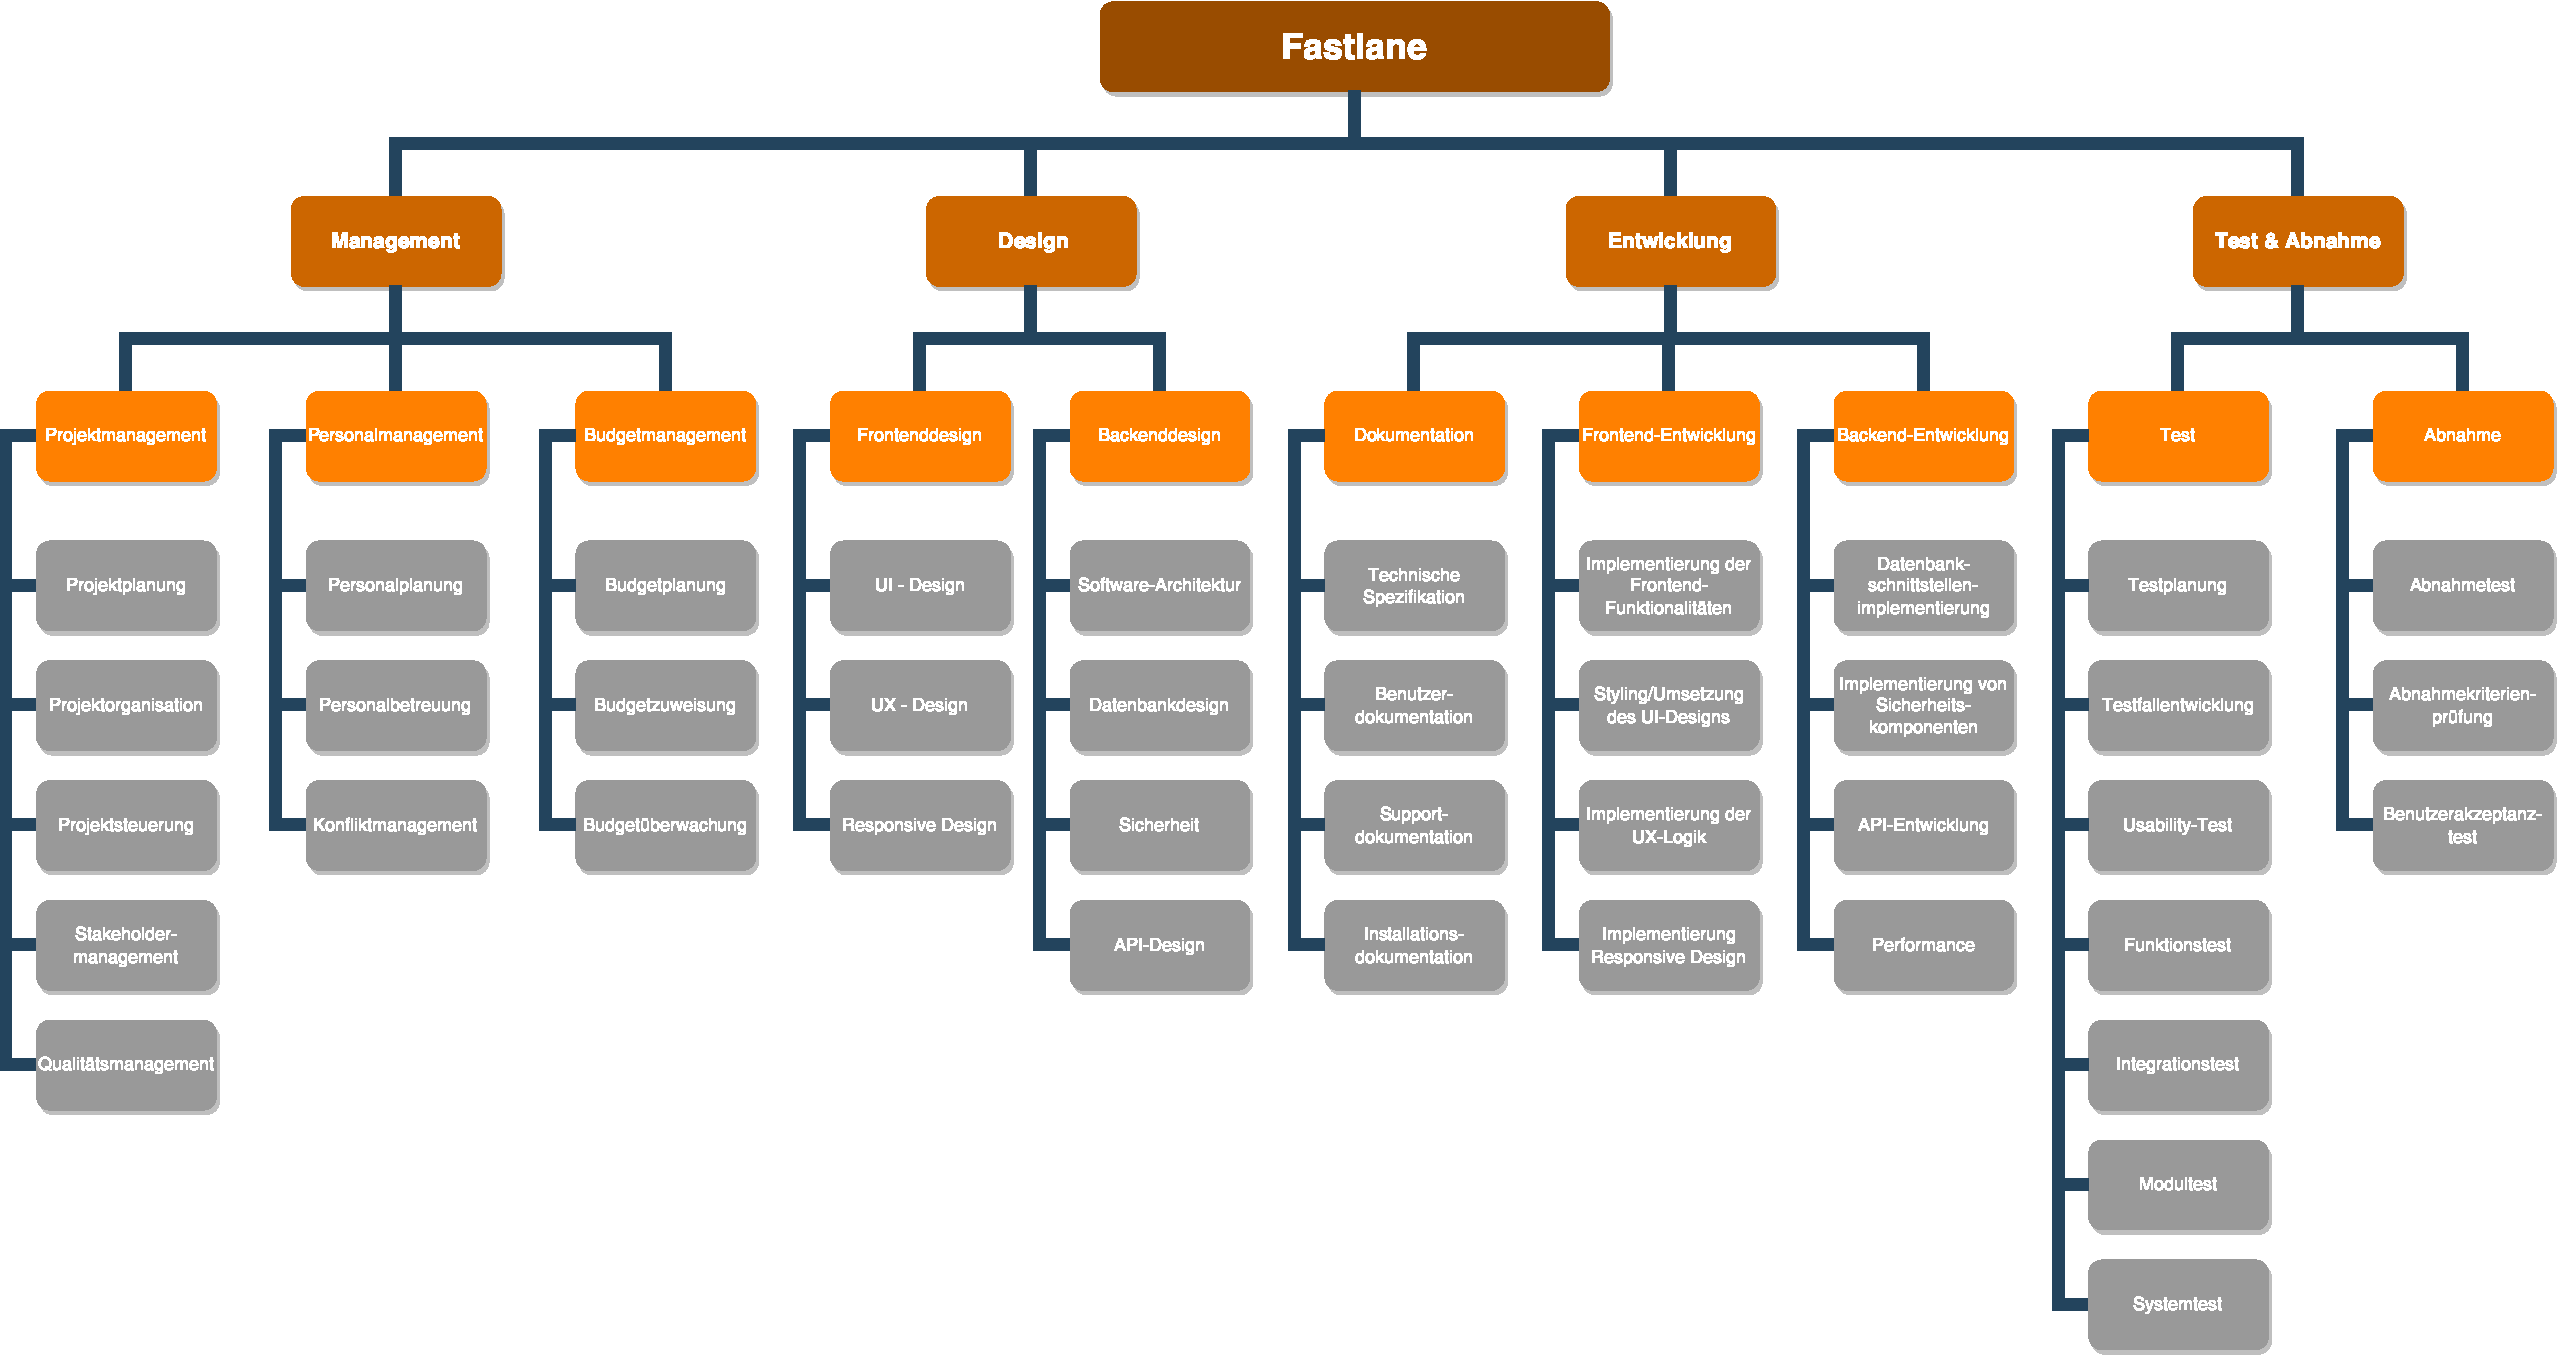
\includegraphics[width = 1.4\textwidth]{pictures/Projektstrukturplan}
        \caption{Disziplinorientierter Projektstrukturplan}
        \label{fig:anwendungsfalldiagramm_2}
    \end{figure}

    \subsection{Projektzeitplan}
    \label{subsec:anhang_projektzeitplan}

    \begin{uml}[H]
        \centering
        % generated by Plantuml 1.2023.7
\definecolor{plantucolor0000}{RGB}{0,0,0}
\definecolor{plantucolor0001}{RGB}{192,192,192}
\definecolor{plantucolor0002}{RGB}{24,24,24}
\definecolor{plantucolor0003}{RGB}{50,168,82}
\definecolor{plantucolor0004}{RGB}{255,255,255}
\definecolor{plantucolor0005}{RGB}{255,255,255}
\definecolor{plantucolor0006}{RGB}{242,146,29}
\definecolor{plantucolor0007}{RGB}{71,114,186}
\definecolor{plantucolor0008}{RGB}{230,168,25}
\scalebox{0.767}{
    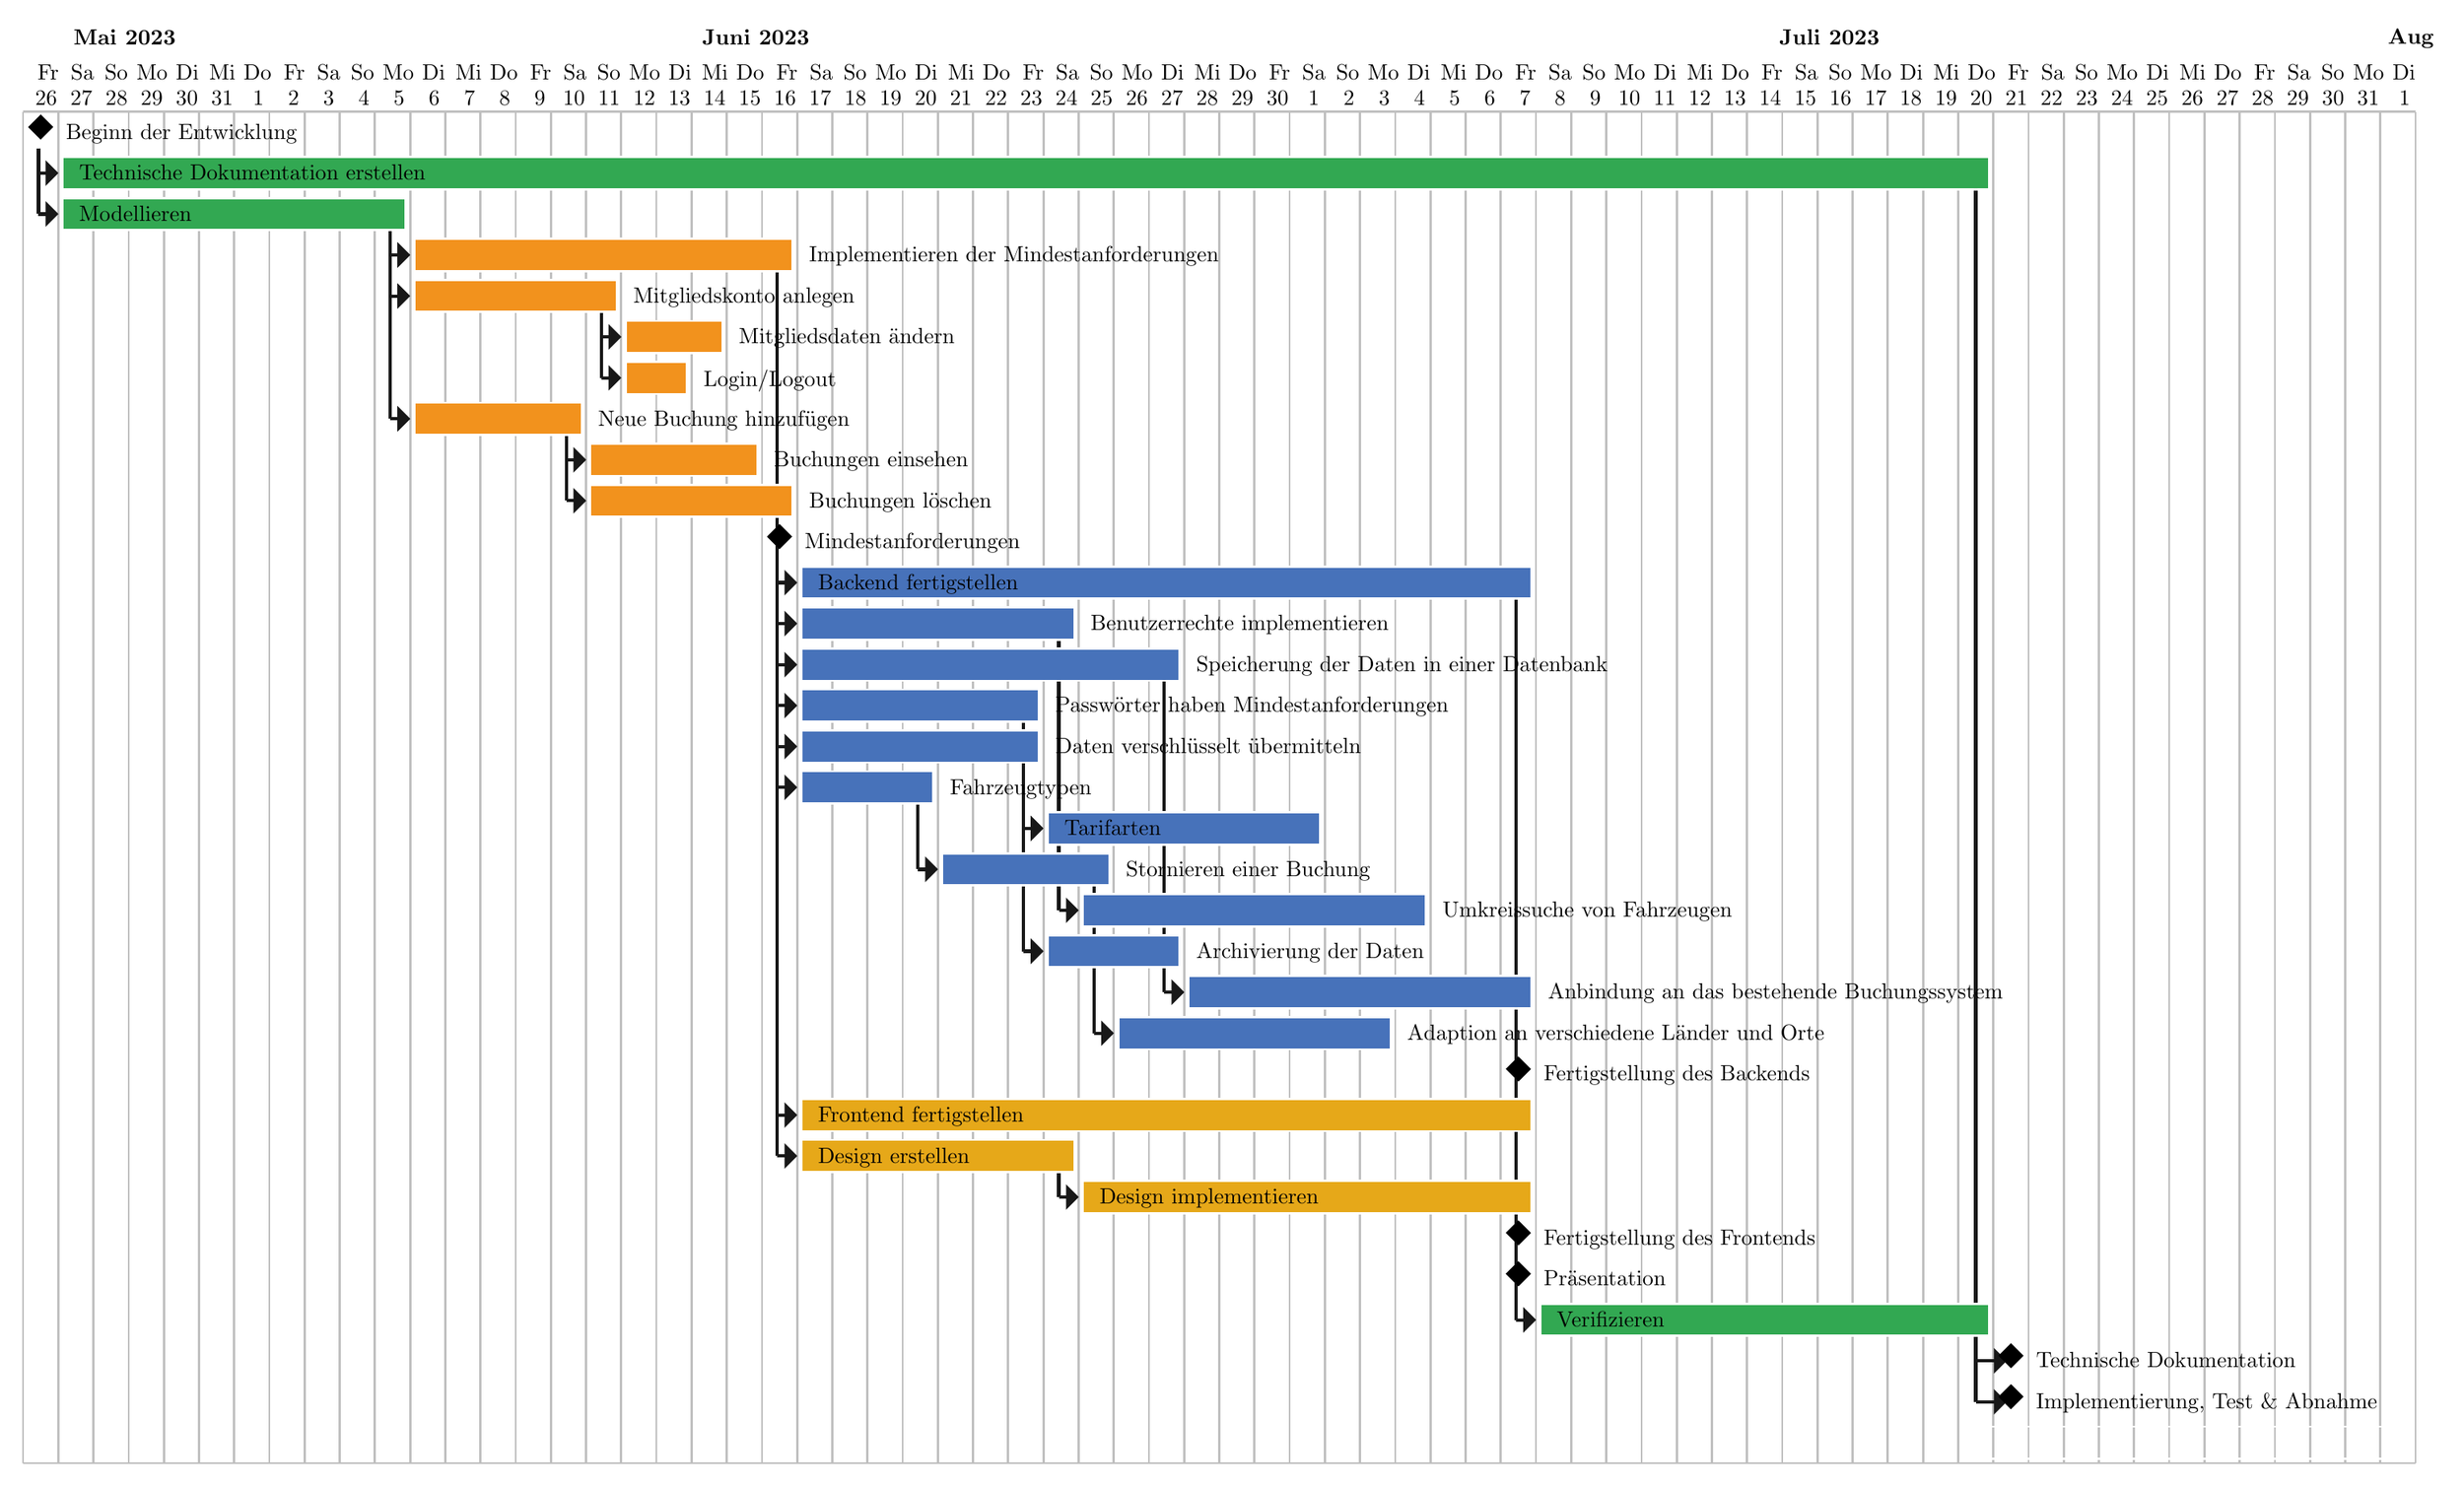
\begin{tikzpicture}[yscale=-1
    ,pstyle0/.style={color=plantucolor0001,line width=1.0pt}
    ,pstyle1/.style={color=plantucolor0002,line width=1.5pt}
    ,pstyle2/.style={color=plantucolor0002,fill=plantucolor0002,line width=1.5pt}
    ,pstyle3/.style={color=black,fill=black,line width=1.0pt}
    ,pstyle4/.style={color=plantucolor0004,fill=plantucolor0003,line width=1.0pt}
    ,pstyle5/.style={color=white,line width=1.0pt}
    ,pstyle6/.style={color=plantucolor0004,fill=plantucolor0006,line width=1.0pt}
    ,pstyle7/.style={color=plantucolor0004,fill=plantucolor0007,line width=1.0pt}
    ,pstyle8/.style={color=plantucolor0004,fill=plantucolor0008,line width=1.0pt}
    ,pstyle9/.style={color=plantucolor0004,line width=1.0pt}
    ]
        \node at (3.0444pt,16pt)[below right,color=black]{Fr};
        \node at (18.2pt,16pt)[below right,color=black]{Sa};
        \node at (33.5818pt,16pt)[below right,color=black]{So};
        \node at (48.0286pt,16pt)[below right,color=black]{Mo};
        \node at (66pt,16pt)[below right,color=black]{Di};
        \node at (81.1333pt,16pt)[below right,color=black]{Mi};
        \node at (96.8pt,16pt)[below right,color=black]{Do};
        \node at (115.0444pt,16pt)[below right,color=black]{Fr};
        \node at (130.2pt,16pt)[below right,color=black]{Sa};
        \node at (145.5818pt,16pt)[below right,color=black]{So};
        \node at (160.0286pt,16pt)[below right,color=black]{Mo};
        \node at (178pt,16pt)[below right,color=black]{Di};
        \node at (193.1333pt,16pt)[below right,color=black]{Mi};
        \node at (208.8pt,16pt)[below right,color=black]{Do};
        \node at (227.0444pt,16pt)[below right,color=black]{Fr};
        \node at (242.2pt,16pt)[below right,color=black]{Sa};
        \node at (257.5818pt,16pt)[below right,color=black]{So};
        \node at (272.0286pt,16pt)[below right,color=black]{Mo};
        \node at (290pt,16pt)[below right,color=black]{Di};
        \node at (305.1333pt,16pt)[below right,color=black]{Mi};
        \node at (320.8pt,16pt)[below right,color=black]{Do};
        \node at (339.0444pt,16pt)[below right,color=black]{Fr};
        \node at (354.2pt,16pt)[below right,color=black]{Sa};
        \node at (369.5818pt,16pt)[below right,color=black]{So};
        \node at (384.0286pt,16pt)[below right,color=black]{Mo};
        \node at (402pt,16pt)[below right,color=black]{Di};
        \node at (417.1333pt,16pt)[below right,color=black]{Mi};
        \node at (432.8pt,16pt)[below right,color=black]{Do};
        \node at (451.0444pt,16pt)[below right,color=black]{Fr};
        \node at (466.2pt,16pt)[below right,color=black]{Sa};
        \node at (481.5818pt,16pt)[below right,color=black]{So};
        \node at (496.0286pt,16pt)[below right,color=black]{Mo};
        \node at (514pt,16pt)[below right,color=black]{Di};
        \node at (529.1333pt,16pt)[below right,color=black]{Mi};
        \node at (544.8pt,16pt)[below right,color=black]{Do};
        \node at (563.0444pt,16pt)[below right,color=black]{Fr};
        \node at (578.2pt,16pt)[below right,color=black]{Sa};
        \node at (593.5818pt,16pt)[below right,color=black]{So};
        \node at (608.0286pt,16pt)[below right,color=black]{Mo};
        \node at (626pt,16pt)[below right,color=black]{Di};
        \node at (641.1333pt,16pt)[below right,color=black]{Mi};
        \node at (656.8pt,16pt)[below right,color=black]{Do};
        \node at (675.0444pt,16pt)[below right,color=black]{Fr};
        \node at (690.2pt,16pt)[below right,color=black]{Sa};
        \node at (705.5818pt,16pt)[below right,color=black]{So};
        \node at (720.0286pt,16pt)[below right,color=black]{Mo};
        \node at (738pt,16pt)[below right,color=black]{Di};
        \node at (753.1333pt,16pt)[below right,color=black]{Mi};
        \node at (768.8pt,16pt)[below right,color=black]{Do};
        \node at (787.0444pt,16pt)[below right,color=black]{Fr};
        \node at (802.2pt,16pt)[below right,color=black]{Sa};
        \node at (817.5818pt,16pt)[below right,color=black]{So};
        \node at (832.0286pt,16pt)[below right,color=black]{Mo};
        \node at (850pt,16pt)[below right,color=black]{Di};
        \node at (865.1333pt,16pt)[below right,color=black]{Mi};
        \node at (880.8pt,16pt)[below right,color=black]{Do};
        \node at (899.0444pt,16pt)[below right,color=black]{Fr};
        \node at (914.2pt,16pt)[below right,color=black]{Sa};
        \node at (929.5818pt,16pt)[below right,color=black]{So};
        \node at (944.0286pt,16pt)[below right,color=black]{Mo};
        \node at (962pt,16pt)[below right,color=black]{Di};
        \node at (977.1333pt,16pt)[below right,color=black]{Mi};
        \node at (992.8pt,16pt)[below right,color=black]{Do};
        \node at (1011.0444pt,16pt)[below right,color=black]{Fr};
        \node at (1026.2pt,16pt)[below right,color=black]{Sa};
        \node at (1041.5818pt,16pt)[below right,color=black]{So};
        \node at (1056.0286pt,16pt)[below right,color=black]{Mo};
        \node at (1074pt,16pt)[below right,color=black]{Di};
        \node at (2pt,28pt)[below right,color=black]{26};
        \node at (18pt,28pt)[below right,color=black]{27};
        \node at (34pt,28pt)[below right,color=black]{28};
        \node at (50pt,28pt)[below right,color=black]{29};
        \node at (66pt,28pt)[below right,color=black]{30};
        \node at (82pt,28pt)[below right,color=black]{31};
        \node at (101pt,28pt)[below right,color=black]{1};
        \node at (117pt,28pt)[below right,color=black]{2};
        \node at (133pt,28pt)[below right,color=black]{3};
        \node at (149pt,28pt)[below right,color=black]{4};
        \node at (165pt,28pt)[below right,color=black]{5};
        \node at (181pt,28pt)[below right,color=black]{6};
        \node at (197pt,28pt)[below right,color=black]{7};
        \node at (213pt,28pt)[below right,color=black]{8};
        \node at (229pt,28pt)[below right,color=black]{9};
        \node at (242pt,28pt)[below right,color=black]{10};
        \node at (258pt,28pt)[below right,color=black]{11};
        \node at (274pt,28pt)[below right,color=black]{12};
        \node at (290pt,28pt)[below right,color=black]{13};
        \node at (306pt,28pt)[below right,color=black]{14};
        \node at (322pt,28pt)[below right,color=black]{15};
        \node at (338pt,28pt)[below right,color=black]{16};
        \node at (354pt,28pt)[below right,color=black]{17};
        \node at (370pt,28pt)[below right,color=black]{18};
        \node at (386pt,28pt)[below right,color=black]{19};
        \node at (402pt,28pt)[below right,color=black]{20};
        \node at (418pt,28pt)[below right,color=black]{21};
        \node at (434pt,28pt)[below right,color=black]{22};
        \node at (450pt,28pt)[below right,color=black]{23};
        \node at (466pt,28pt)[below right,color=black]{24};
        \node at (482pt,28pt)[below right,color=black]{25};
        \node at (498pt,28pt)[below right,color=black]{26};
        \node at (514pt,28pt)[below right,color=black]{27};
        \node at (530pt,28pt)[below right,color=black]{28};
        \node at (546pt,28pt)[below right,color=black]{29};
        \node at (562pt,28pt)[below right,color=black]{30};
        \node at (581pt,28pt)[below right,color=black]{1};
        \node at (597pt,28pt)[below right,color=black]{2};
        \node at (613pt,28pt)[below right,color=black]{3};
        \node at (629pt,28pt)[below right,color=black]{4};
        \node at (645pt,28pt)[below right,color=black]{5};
        \node at (661pt,28pt)[below right,color=black]{6};
        \node at (677pt,28pt)[below right,color=black]{7};
        \node at (693pt,28pt)[below right,color=black]{8};
        \node at (709pt,28pt)[below right,color=black]{9};
        \node at (722pt,28pt)[below right,color=black]{10};
        \node at (738pt,28pt)[below right,color=black]{11};
        \node at (754pt,28pt)[below right,color=black]{12};
        \node at (770pt,28pt)[below right,color=black]{13};
        \node at (786pt,28pt)[below right,color=black]{14};
        \node at (802pt,28pt)[below right,color=black]{15};
        \node at (818pt,28pt)[below right,color=black]{16};
        \node at (834pt,28pt)[below right,color=black]{17};
        \node at (850pt,28pt)[below right,color=black]{18};
        \node at (866pt,28pt)[below right,color=black]{19};
        \node at (882pt,28pt)[below right,color=black]{20};
        \node at (898pt,28pt)[below right,color=black]{21};
        \node at (914pt,28pt)[below right,color=black]{22};
        \node at (930pt,28pt)[below right,color=black]{23};
        \node at (946pt,28pt)[below right,color=black]{24};
        \node at (962pt,28pt)[below right,color=black]{25};
        \node at (978pt,28pt)[below right,color=black]{26};
        \node at (994pt,28pt)[below right,color=black]{27};
        \node at (1010pt,28pt)[below right,color=black]{28};
        \node at (1026pt,28pt)[below right,color=black]{29};
        \node at (1042pt,28pt)[below right,color=black]{30};
        \node at (1058pt,28pt)[below right,color=black]{31};
        \node at (1077pt,28pt)[below right,color=black]{1};
        \node at (19.4083pt,0pt)[below right,color=black]{\textbf{Mai 2023}};
        \node at (305.4pt,0pt)[below right,color=black]{\textbf{Juni 2023}};
        \node at (795.2pt,0pt)[below right,color=black]{\textbf{Juli 2023}};
        \node at (1072pt,0pt)[below right,color=black]{\textbf{Aug}};
        \draw[pstyle0] (0pt,41pt) -- (0pt,655.8184pt);
        \draw[pstyle0] (16pt,41pt) -- (16pt,655.8184pt);
        \draw[pstyle0] (32pt,41pt) -- (32pt,655.8184pt);
        \draw[pstyle0] (48pt,41pt) -- (48pt,655.8184pt);
        \draw[pstyle0] (64pt,41pt) -- (64pt,655.8184pt);
        \draw[pstyle0] (80pt,41pt) -- (80pt,655.8184pt);
        \draw[pstyle0] (96pt,41pt) -- (96pt,655.8184pt);
        \draw[pstyle0] (112pt,41pt) -- (112pt,655.8184pt);
        \draw[pstyle0] (128pt,41pt) -- (128pt,655.8184pt);
        \draw[pstyle0] (144pt,41pt) -- (144pt,655.8184pt);
        \draw[pstyle0] (160pt,41pt) -- (160pt,655.8184pt);
        \draw[pstyle0] (176pt,41pt) -- (176pt,655.8184pt);
        \draw[pstyle0] (192pt,41pt) -- (192pt,655.8184pt);
        \draw[pstyle0] (208pt,41pt) -- (208pt,655.8184pt);
        \draw[pstyle0] (224pt,41pt) -- (224pt,655.8184pt);
        \draw[pstyle0] (240pt,41pt) -- (240pt,655.8184pt);
        \draw[pstyle0] (256pt,41pt) -- (256pt,655.8184pt);
        \draw[pstyle0] (272pt,41pt) -- (272pt,655.8184pt);
        \draw[pstyle0] (288pt,41pt) -- (288pt,655.8184pt);
        \draw[pstyle0] (304pt,41pt) -- (304pt,655.8184pt);
        \draw[pstyle0] (320pt,41pt) -- (320pt,655.8184pt);
        \draw[pstyle0] (336pt,41pt) -- (336pt,655.8184pt);
        \draw[pstyle0] (352pt,41pt) -- (352pt,655.8184pt);
        \draw[pstyle0] (368pt,41pt) -- (368pt,655.8184pt);
        \draw[pstyle0] (384pt,41pt) -- (384pt,655.8184pt);
        \draw[pstyle0] (400pt,41pt) -- (400pt,655.8184pt);
        \draw[pstyle0] (416pt,41pt) -- (416pt,655.8184pt);
        \draw[pstyle0] (432pt,41pt) -- (432pt,655.8184pt);
        \draw[pstyle0] (448pt,41pt) -- (448pt,655.8184pt);
        \draw[pstyle0] (464pt,41pt) -- (464pt,655.8184pt);
        \draw[pstyle0] (480pt,41pt) -- (480pt,655.8184pt);
        \draw[pstyle0] (496pt,41pt) -- (496pt,655.8184pt);
        \draw[pstyle0] (512pt,41pt) -- (512pt,655.8184pt);
        \draw[pstyle0] (528pt,41pt) -- (528pt,655.8184pt);
        \draw[pstyle0] (544pt,41pt) -- (544pt,655.8184pt);
        \draw[pstyle0] (560pt,41pt) -- (560pt,655.8184pt);
        \draw[pstyle0] (576pt,41pt) -- (576pt,655.8184pt);
        \draw[pstyle0] (592pt,41pt) -- (592pt,655.8184pt);
        \draw[pstyle0] (608pt,41pt) -- (608pt,655.8184pt);
        \draw[pstyle0] (624pt,41pt) -- (624pt,655.8184pt);
        \draw[pstyle0] (640pt,41pt) -- (640pt,655.8184pt);
        \draw[pstyle0] (656pt,41pt) -- (656pt,655.8184pt);
        \draw[pstyle0] (672pt,41pt) -- (672pt,655.8184pt);
        \draw[pstyle0] (688pt,41pt) -- (688pt,655.8184pt);
        \draw[pstyle0] (704pt,41pt) -- (704pt,655.8184pt);
        \draw[pstyle0] (720pt,41pt) -- (720pt,655.8184pt);
        \draw[pstyle0] (736pt,41pt) -- (736pt,655.8184pt);
        \draw[pstyle0] (752pt,41pt) -- (752pt,655.8184pt);
        \draw[pstyle0] (768pt,41pt) -- (768pt,655.8184pt);
        \draw[pstyle0] (784pt,41pt) -- (784pt,655.8184pt);
        \draw[pstyle0] (800pt,41pt) -- (800pt,655.8184pt);
        \draw[pstyle0] (816pt,41pt) -- (816pt,655.8184pt);
        \draw[pstyle0] (832pt,41pt) -- (832pt,655.8184pt);
        \draw[pstyle0] (848pt,41pt) -- (848pt,655.8184pt);
        \draw[pstyle0] (864pt,41pt) -- (864pt,655.8184pt);
        \draw[pstyle0] (880pt,41pt) -- (880pt,655.8184pt);
        \draw[pstyle0] (896pt,41pt) -- (896pt,655.8184pt);
        \draw[pstyle0] (912pt,41pt) -- (912pt,655.8184pt);
        \draw[pstyle0] (928pt,41pt) -- (928pt,655.8184pt);
        \draw[pstyle0] (944pt,41pt) -- (944pt,655.8184pt);
        \draw[pstyle0] (960pt,41pt) -- (960pt,655.8184pt);
        \draw[pstyle0] (976pt,41pt) -- (976pt,655.8184pt);
        \draw[pstyle0] (992pt,41pt) -- (992pt,655.8184pt);
        \draw[pstyle0] (1008pt,41pt) -- (1008pt,655.8184pt);
        \draw[pstyle0] (1024pt,41pt) -- (1024pt,655.8184pt);
        \draw[pstyle0] (1040pt,41pt) -- (1040pt,655.8184pt);
        \draw[pstyle0] (1056pt,41pt) -- (1056pt,655.8184pt);
        \draw[pstyle0] (1072pt,41pt) -- (1072pt,655.8184pt);
        \draw[pstyle0] (1088pt,41pt) -- (1088pt,655.8184pt);
        \draw[pstyle0] (0pt,41pt) -- (1088pt,41pt);
        \draw[pstyle0] (0pt,655.8184pt) -- (1088pt,655.8184pt);
        \draw[pstyle1] (7pt,57.6309pt) -- (7pt,68.9463pt);
        \draw[pstyle1] (7pt,68.9463pt) -- (15pt,68.9463pt);
        \draw[pstyle2] (11pt,64.9463pt) -- (11pt,68.9463pt) -- (11pt,72.9463pt) -- (15pt,68.9463pt) -- cycle;
        \draw[pstyle1] (7pt,57.6309pt) -- (7pt,87.5771pt);
        \draw[pstyle1] (7pt,87.5771pt) -- (15pt,87.5771pt);
        \draw[pstyle2] (11pt,83.5771pt) -- (11pt,87.5771pt) -- (11pt,91.5771pt) -- (15pt,87.5771pt) -- cycle;
        \draw[pstyle1] (167pt,94.8926pt) -- (167pt,106.208pt);
        \draw[pstyle1] (167pt,106.208pt) -- (175pt,106.208pt);
        \draw[pstyle2] (171pt,102.208pt) -- (171pt,106.208pt) -- (171pt,110.208pt) -- (175pt,106.208pt) -- cycle;
        \draw[pstyle1] (167pt,94.8926pt) -- (167pt,124.8389pt);
        \draw[pstyle1] (167pt,124.8389pt) -- (175pt,124.8389pt);
        \draw[pstyle2] (171pt,120.8389pt) -- (171pt,124.8389pt) -- (171pt,128.8389pt) -- (175pt,124.8389pt) -- cycle;
        \draw[pstyle1] (263pt,132.1543pt) -- (263pt,143.4697pt);
        \draw[pstyle1] (263pt,143.4697pt) -- (271pt,143.4697pt);
        \draw[pstyle2] (267pt,139.4697pt) -- (267pt,143.4697pt) -- (267pt,147.4697pt) -- (271pt,143.4697pt) -- cycle;
        \draw[pstyle1] (263pt,132.1543pt) -- (263pt,162.1006pt);
        \draw[pstyle1] (263pt,162.1006pt) -- (271pt,162.1006pt);
        \draw[pstyle2] (267pt,158.1006pt) -- (267pt,162.1006pt) -- (267pt,166.1006pt) -- (271pt,162.1006pt) -- cycle;
        \draw[pstyle1] (167pt,94.8926pt) -- (167pt,180.7314pt);
        \draw[pstyle1] (167pt,180.7314pt) -- (175pt,180.7314pt);
        \draw[pstyle2] (171pt,176.7314pt) -- (171pt,180.7314pt) -- (171pt,184.7314pt) -- (175pt,180.7314pt) -- cycle;
        \draw[pstyle1] (247pt,188.0469pt) -- (247pt,199.3623pt);
        \draw[pstyle1] (247pt,199.3623pt) -- (255pt,199.3623pt);
        \draw[pstyle2] (251pt,195.3623pt) -- (251pt,199.3623pt) -- (251pt,203.3623pt) -- (255pt,199.3623pt) -- cycle;
        \draw[pstyle1] (247pt,188.0469pt) -- (247pt,217.9932pt);
        \draw[pstyle1] (247pt,217.9932pt) -- (255pt,217.9932pt);
        \draw[pstyle2] (251pt,213.9932pt) -- (251pt,217.9932pt) -- (251pt,221.9932pt) -- (255pt,217.9932pt) -- cycle;
        \draw[pstyle1] (343pt,113.5234pt) -- (343pt,255.2549pt);
        \draw[pstyle1] (343pt,255.2549pt) -- (351pt,255.2549pt);
        \draw[pstyle2] (347pt,251.2549pt) -- (347pt,255.2549pt) -- (347pt,259.2549pt) -- (351pt,255.2549pt) -- cycle;
        \draw[pstyle1] (343pt,113.5234pt) -- (343pt,273.8857pt);
        \draw[pstyle1] (343pt,273.8857pt) -- (351pt,273.8857pt);
        \draw[pstyle2] (347pt,269.8857pt) -- (347pt,273.8857pt) -- (347pt,277.8857pt) -- (351pt,273.8857pt) -- cycle;
        \draw[pstyle1] (343pt,113.5234pt) -- (343pt,292.5166pt);
        \draw[pstyle1] (343pt,292.5166pt) -- (351pt,292.5166pt);
        \draw[pstyle2] (347pt,288.5166pt) -- (347pt,292.5166pt) -- (347pt,296.5166pt) -- (351pt,292.5166pt) -- cycle;
        \draw[pstyle1] (343pt,113.5234pt) -- (343pt,311.1475pt);
        \draw[pstyle1] (343pt,311.1475pt) -- (351pt,311.1475pt);
        \draw[pstyle2] (347pt,307.1475pt) -- (347pt,311.1475pt) -- (347pt,315.1475pt) -- (351pt,311.1475pt) -- cycle;
        \draw[pstyle1] (343pt,113.5234pt) -- (343pt,329.7783pt);
        \draw[pstyle1] (343pt,329.7783pt) -- (351pt,329.7783pt);
        \draw[pstyle2] (347pt,325.7783pt) -- (347pt,329.7783pt) -- (347pt,333.7783pt) -- (351pt,329.7783pt) -- cycle;
        \draw[pstyle1] (343pt,113.5234pt) -- (343pt,348.4092pt);
        \draw[pstyle1] (343pt,348.4092pt) -- (351pt,348.4092pt);
        \draw[pstyle2] (347pt,344.4092pt) -- (347pt,348.4092pt) -- (347pt,352.4092pt) -- (351pt,348.4092pt) -- cycle;
        \draw[pstyle1] (455pt,318.4629pt) -- (455pt,367.04pt);
        \draw[pstyle1] (455pt,367.04pt) -- (463pt,367.04pt);
        \draw[pstyle2] (459pt,363.04pt) -- (459pt,367.04pt) -- (459pt,371.04pt) -- (463pt,367.04pt) -- cycle;
        \draw[pstyle1] (407pt,355.7246pt) -- (407pt,385.6709pt);
        \draw[pstyle1] (407pt,385.6709pt) -- (415pt,385.6709pt);
        \draw[pstyle2] (411pt,381.6709pt) -- (411pt,385.6709pt) -- (411pt,389.6709pt) -- (415pt,385.6709pt) -- cycle;
        \draw[pstyle1] (471pt,281.2012pt) -- (471pt,404.3018pt);
        \draw[pstyle1] (471pt,404.3018pt) -- (479pt,404.3018pt);
        \draw[pstyle2] (475pt,400.3018pt) -- (475pt,404.3018pt) -- (475pt,408.3018pt) -- (479pt,404.3018pt) -- cycle;
        \draw[pstyle1] (455pt,337.0938pt) -- (455pt,422.9326pt);
        \draw[pstyle1] (455pt,422.9326pt) -- (463pt,422.9326pt);
        \draw[pstyle2] (459pt,418.9326pt) -- (459pt,422.9326pt) -- (459pt,426.9326pt) -- (463pt,422.9326pt) -- cycle;
        \draw[pstyle1] (519pt,299.832pt) -- (519pt,441.5635pt);
        \draw[pstyle1] (519pt,441.5635pt) -- (527pt,441.5635pt);
        \draw[pstyle2] (523pt,437.5635pt) -- (523pt,441.5635pt) -- (523pt,445.5635pt) -- (527pt,441.5635pt) -- cycle;
        \draw[pstyle1] (487pt,392.9863pt) -- (487pt,460.1943pt);
        \draw[pstyle1] (487pt,460.1943pt) -- (495pt,460.1943pt);
        \draw[pstyle2] (491pt,456.1943pt) -- (491pt,460.1943pt) -- (491pt,464.1943pt) -- (495pt,460.1943pt) -- cycle;
        \draw[pstyle1] (343pt,113.5234pt) -- (343pt,497.4561pt);
        \draw[pstyle1] (343pt,497.4561pt) -- (351pt,497.4561pt);
        \draw[pstyle2] (347pt,493.4561pt) -- (347pt,497.4561pt) -- (347pt,501.4561pt) -- (351pt,497.4561pt) -- cycle;
        \draw[pstyle1] (343pt,113.5234pt) -- (343pt,516.0869pt);
        \draw[pstyle1] (343pt,516.0869pt) -- (351pt,516.0869pt);
        \draw[pstyle2] (347pt,512.0869pt) -- (347pt,516.0869pt) -- (347pt,520.0869pt) -- (351pt,516.0869pt) -- cycle;
        \draw[pstyle1] (471pt,523.4023pt) -- (471pt,534.7178pt);
        \draw[pstyle1] (471pt,534.7178pt) -- (479pt,534.7178pt);
        \draw[pstyle2] (475pt,530.7178pt) -- (475pt,534.7178pt) -- (475pt,538.7178pt) -- (479pt,534.7178pt) -- cycle;
        \draw[pstyle1] (679pt,262.5703pt) -- (679pt,590.6104pt);
        \draw[pstyle1] (679pt,590.6104pt) -- (687pt,590.6104pt);
        \draw[pstyle2] (683pt,586.6104pt) -- (683pt,590.6104pt) -- (683pt,594.6104pt) -- (687pt,590.6104pt) -- cycle;
        \draw[pstyle1] (888pt,76.2617pt) -- (888pt,609.2412pt);
        \draw[pstyle1] (888pt,609.2412pt) -- (901pt,609.2412pt);
        \draw[pstyle2] (897pt,605.2412pt) -- (897pt,609.2412pt) -- (897pt,613.2412pt) -- (901pt,609.2412pt) -- cycle;
        \draw[pstyle1] (888pt,76.2617pt) -- (888pt,627.8721pt);
        \draw[pstyle1] (888pt,627.8721pt) -- (901pt,627.8721pt);
        \draw[pstyle2] (897pt,623.8721pt) -- (897pt,627.8721pt) -- (897pt,631.8721pt) -- (901pt,627.8721pt) -- cycle;
        \draw[pstyle3] (8pt,43pt) -- (13pt,48pt) -- (8pt,53pt) -- (3pt,48pt) -- cycle;
        \draw[pstyle4] (18pt,61.6309pt) rectangle (894pt,76.2617pt);
        \draw[pstyle5] (18pt,61.6309pt) -- (894pt,61.6309pt);
        \draw[pstyle5] (18pt,76.2617pt) -- (894pt,76.2617pt);
        \draw[pstyle5] (18pt,61.6309pt) -- (18pt,76.2617pt);
        \draw[pstyle5] (894pt,61.6309pt) -- (894pt,76.2617pt);
        \draw[pstyle4] (18pt,80.2617pt) rectangle (174pt,94.8926pt);
        \draw[pstyle5] (18pt,80.2617pt) -- (174pt,80.2617pt);
        \draw[pstyle5] (18pt,94.8926pt) -- (174pt,94.8926pt);
        \draw[pstyle5] (18pt,80.2617pt) -- (18pt,94.8926pt);
        \draw[pstyle5] (174pt,80.2617pt) -- (174pt,94.8926pt);
        \draw[pstyle6] (178pt,98.8926pt) rectangle (350pt,113.5234pt);
        \draw[pstyle5] (178pt,98.8926pt) -- (350pt,98.8926pt);
        \draw[pstyle5] (178pt,113.5234pt) -- (350pt,113.5234pt);
        \draw[pstyle5] (178pt,98.8926pt) -- (178pt,113.5234pt);
        \draw[pstyle5] (350pt,98.8926pt) -- (350pt,113.5234pt);
        \draw[pstyle6] (178pt,117.5234pt) rectangle (270pt,132.1543pt);
        \draw[pstyle5] (178pt,117.5234pt) -- (270pt,117.5234pt);
        \draw[pstyle5] (178pt,132.1543pt) -- (270pt,132.1543pt);
        \draw[pstyle5] (178pt,117.5234pt) -- (178pt,132.1543pt);
        \draw[pstyle5] (270pt,117.5234pt) -- (270pt,132.1543pt);
        \draw[pstyle6] (274pt,136.1543pt) rectangle (318pt,150.7852pt);
        \draw[pstyle5] (274pt,136.1543pt) -- (318pt,136.1543pt);
        \draw[pstyle5] (274pt,150.7852pt) -- (318pt,150.7852pt);
        \draw[pstyle5] (274pt,136.1543pt) -- (274pt,150.7852pt);
        \draw[pstyle5] (318pt,136.1543pt) -- (318pt,150.7852pt);
        \draw[pstyle6] (274pt,154.7852pt) rectangle (302pt,169.416pt);
        \draw[pstyle5] (274pt,154.7852pt) -- (302pt,154.7852pt);
        \draw[pstyle5] (274pt,169.416pt) -- (302pt,169.416pt);
        \draw[pstyle5] (274pt,154.7852pt) -- (274pt,169.416pt);
        \draw[pstyle5] (302pt,154.7852pt) -- (302pt,169.416pt);
        \draw[pstyle6] (178pt,173.416pt) rectangle (254pt,188.0469pt);
        \draw[pstyle5] (178pt,173.416pt) -- (254pt,173.416pt);
        \draw[pstyle5] (178pt,188.0469pt) -- (254pt,188.0469pt);
        \draw[pstyle5] (178pt,173.416pt) -- (178pt,188.0469pt);
        \draw[pstyle5] (254pt,173.416pt) -- (254pt,188.0469pt);
        \draw[pstyle6] (258pt,192.0469pt) rectangle (334pt,206.6777pt);
        \draw[pstyle5] (258pt,192.0469pt) -- (334pt,192.0469pt);
        \draw[pstyle5] (258pt,206.6777pt) -- (334pt,206.6777pt);
        \draw[pstyle5] (258pt,192.0469pt) -- (258pt,206.6777pt);
        \draw[pstyle5] (334pt,192.0469pt) -- (334pt,206.6777pt);
        \draw[pstyle6] (258pt,210.6777pt) rectangle (350pt,225.3086pt);
        \draw[pstyle5] (258pt,210.6777pt) -- (350pt,210.6777pt);
        \draw[pstyle5] (258pt,225.3086pt) -- (350pt,225.3086pt);
        \draw[pstyle5] (258pt,210.6777pt) -- (258pt,225.3086pt);
        \draw[pstyle5] (350pt,210.6777pt) -- (350pt,225.3086pt);
        \draw[pstyle3] (344pt,229.3086pt) -- (349pt,234.3086pt) -- (344pt,239.3086pt) -- (339pt,234.3086pt) -- cycle;
        \draw[pstyle7] (354pt,247.9395pt) rectangle (686pt,262.5703pt);
        \draw[pstyle5] (354pt,247.9395pt) -- (686pt,247.9395pt);
        \draw[pstyle5] (354pt,262.5703pt) -- (686pt,262.5703pt);
        \draw[pstyle5] (354pt,247.9395pt) -- (354pt,262.5703pt);
        \draw[pstyle5] (686pt,247.9395pt) -- (686pt,262.5703pt);
        \draw[pstyle7] (354pt,266.5703pt) rectangle (478pt,281.2012pt);
        \draw[pstyle5] (354pt,266.5703pt) -- (478pt,266.5703pt);
        \draw[pstyle5] (354pt,281.2012pt) -- (478pt,281.2012pt);
        \draw[pstyle5] (354pt,266.5703pt) -- (354pt,281.2012pt);
        \draw[pstyle5] (478pt,266.5703pt) -- (478pt,281.2012pt);
        \draw[pstyle7] (354pt,285.2012pt) rectangle (526pt,299.832pt);
        \draw[pstyle5] (354pt,285.2012pt) -- (526pt,285.2012pt);
        \draw[pstyle5] (354pt,299.832pt) -- (526pt,299.832pt);
        \draw[pstyle5] (354pt,285.2012pt) -- (354pt,299.832pt);
        \draw[pstyle5] (526pt,285.2012pt) -- (526pt,299.832pt);
        \draw[pstyle7] (354pt,303.832pt) rectangle (462pt,318.4629pt);
        \draw[pstyle5] (354pt,303.832pt) -- (462pt,303.832pt);
        \draw[pstyle5] (354pt,318.4629pt) -- (462pt,318.4629pt);
        \draw[pstyle5] (354pt,303.832pt) -- (354pt,318.4629pt);
        \draw[pstyle5] (462pt,303.832pt) -- (462pt,318.4629pt);
        \draw[pstyle7] (354pt,322.4629pt) rectangle (462pt,337.0938pt);
        \draw[pstyle5] (354pt,322.4629pt) -- (462pt,322.4629pt);
        \draw[pstyle5] (354pt,337.0938pt) -- (462pt,337.0938pt);
        \draw[pstyle5] (354pt,322.4629pt) -- (354pt,337.0938pt);
        \draw[pstyle5] (462pt,322.4629pt) -- (462pt,337.0938pt);
        \draw[pstyle7] (354pt,341.0938pt) rectangle (414pt,355.7246pt);
        \draw[pstyle5] (354pt,341.0938pt) -- (414pt,341.0938pt);
        \draw[pstyle5] (354pt,355.7246pt) -- (414pt,355.7246pt);
        \draw[pstyle5] (354pt,341.0938pt) -- (354pt,355.7246pt);
        \draw[pstyle5] (414pt,341.0938pt) -- (414pt,355.7246pt);
        \draw[pstyle7] (466pt,359.7246pt) rectangle (590pt,374.3555pt);
        \draw[pstyle5] (466pt,359.7246pt) -- (590pt,359.7246pt);
        \draw[pstyle5] (466pt,374.3555pt) -- (590pt,374.3555pt);
        \draw[pstyle5] (466pt,359.7246pt) -- (466pt,374.3555pt);
        \draw[pstyle5] (590pt,359.7246pt) -- (590pt,374.3555pt);
        \draw[pstyle7] (418pt,378.3555pt) rectangle (494pt,392.9863pt);
        \draw[pstyle5] (418pt,378.3555pt) -- (494pt,378.3555pt);
        \draw[pstyle5] (418pt,392.9863pt) -- (494pt,392.9863pt);
        \draw[pstyle5] (418pt,378.3555pt) -- (418pt,392.9863pt);
        \draw[pstyle5] (494pt,378.3555pt) -- (494pt,392.9863pt);
        \draw[pstyle7] (482pt,396.9863pt) rectangle (638pt,411.6172pt);
        \draw[pstyle5] (482pt,396.9863pt) -- (638pt,396.9863pt);
        \draw[pstyle5] (482pt,411.6172pt) -- (638pt,411.6172pt);
        \draw[pstyle5] (482pt,396.9863pt) -- (482pt,411.6172pt);
        \draw[pstyle5] (638pt,396.9863pt) -- (638pt,411.6172pt);
        \draw[pstyle7] (466pt,415.6172pt) rectangle (526pt,430.248pt);
        \draw[pstyle5] (466pt,415.6172pt) -- (526pt,415.6172pt);
        \draw[pstyle5] (466pt,430.248pt) -- (526pt,430.248pt);
        \draw[pstyle5] (466pt,415.6172pt) -- (466pt,430.248pt);
        \draw[pstyle5] (526pt,415.6172pt) -- (526pt,430.248pt);
        \draw[pstyle7] (530pt,434.248pt) rectangle (686pt,448.8789pt);
        \draw[pstyle5] (530pt,434.248pt) -- (686pt,434.248pt);
        \draw[pstyle5] (530pt,448.8789pt) -- (686pt,448.8789pt);
        \draw[pstyle5] (530pt,434.248pt) -- (530pt,448.8789pt);
        \draw[pstyle5] (686pt,434.248pt) -- (686pt,448.8789pt);
        \draw[pstyle7] (498pt,452.8789pt) rectangle (622pt,467.5098pt);
        \draw[pstyle5] (498pt,452.8789pt) -- (622pt,452.8789pt);
        \draw[pstyle5] (498pt,467.5098pt) -- (622pt,467.5098pt);
        \draw[pstyle5] (498pt,452.8789pt) -- (498pt,467.5098pt);
        \draw[pstyle5] (622pt,452.8789pt) -- (622pt,467.5098pt);
        \draw[pstyle3] (680pt,471.5098pt) -- (685pt,476.5098pt) -- (680pt,481.5098pt) -- (675pt,476.5098pt) -- cycle;
        \draw[pstyle8] (354pt,490.1406pt) rectangle (686pt,504.7715pt);
        \draw[pstyle5] (354pt,490.1406pt) -- (686pt,490.1406pt);
        \draw[pstyle5] (354pt,504.7715pt) -- (686pt,504.7715pt);
        \draw[pstyle5] (354pt,490.1406pt) -- (354pt,504.7715pt);
        \draw[pstyle5] (686pt,490.1406pt) -- (686pt,504.7715pt);
        \draw[pstyle8] (354pt,508.7715pt) rectangle (478pt,523.4023pt);
        \draw[pstyle5] (354pt,508.7715pt) -- (478pt,508.7715pt);
        \draw[pstyle5] (354pt,523.4023pt) -- (478pt,523.4023pt);
        \draw[pstyle5] (354pt,508.7715pt) -- (354pt,523.4023pt);
        \draw[pstyle5] (478pt,508.7715pt) -- (478pt,523.4023pt);
        \draw[pstyle8] (482pt,527.4023pt) rectangle (686pt,542.0332pt);
        \draw[pstyle5] (482pt,527.4023pt) -- (686pt,527.4023pt);
        \draw[pstyle5] (482pt,542.0332pt) -- (686pt,542.0332pt);
        \draw[pstyle5] (482pt,527.4023pt) -- (482pt,542.0332pt);
        \draw[pstyle5] (686pt,527.4023pt) -- (686pt,542.0332pt);
        \draw[pstyle3] (680pt,546.0332pt) -- (685pt,551.0332pt) -- (680pt,556.0332pt) -- (675pt,551.0332pt) -- cycle;
        \draw[pstyle3] (680pt,564.6641pt) -- (685pt,569.6641pt) -- (680pt,574.6641pt) -- (675pt,569.6641pt) -- cycle;
        \draw[pstyle4] (690pt,583.2949pt) rectangle (894pt,597.9258pt);
        \draw[pstyle5] (690pt,583.2949pt) -- (894pt,583.2949pt);
        \draw[pstyle5] (690pt,597.9258pt) -- (894pt,597.9258pt);
        \draw[pstyle5] (690pt,583.2949pt) -- (690pt,597.9258pt);
        \draw[pstyle5] (894pt,583.2949pt) -- (894pt,597.9258pt);
        \draw[pstyle3] (904pt,601.9258pt) -- (909pt,606.9258pt) -- (904pt,611.9258pt) -- (899pt,606.9258pt) -- cycle;
        \draw[pstyle3] (904pt,620.5566pt) -- (909pt,625.5566pt) -- (904pt,630.5566pt) -- (899pt,625.5566pt) -- cycle;
        \draw[pstyle9] (882pt,639.1875pt) rectangle (1086pt,653.8184pt);
        \draw[pstyle9] (882pt,639.1875pt) -- (1086pt,639.1875pt);
        \draw[pstyle9] (882pt,653.8184pt) -- (1086pt,653.8184pt);
        \draw[pstyle9] (882pt,639.1875pt) -- (882pt,653.8184pt);
        \draw[pstyle9] (1086pt,639.1875pt) -- (1086pt,653.8184pt);
        \node at (16pt,43pt)[below right,color=black]{Beginn der Entwicklung};
        \node at (22pt,61.6309pt)[below right,color=black]{Technische Dokumentation erstellen};
        \node at (22pt,80.2617pt)[below right,color=black]{Modellieren};
        \node at (354pt,98.8926pt)[below right,color=black]{Implementieren der Mindestanforderungen};
        \node at (274pt,117.5234pt)[below right,color=black]{Mitgliedskonto anlegen};
        \node at (322pt,136.1543pt)[below right,color=black]{Mitgliedsdaten ändern};
        \node at (306pt,154.7852pt)[below right,color=black]{Login/Logout};
        \node at (258pt,173.416pt)[below right,color=black]{Neue Buchung hinzufügen};
        \node at (338pt,192.0469pt)[below right,color=black]{Buchungen einsehen};
        \node at (354pt,210.6777pt)[below right,color=black]{Buchungen löschen};
        \node at (352pt,229.3086pt)[below right,color=black]{Mindestanforderungen};
        \node at (358pt,247.9395pt)[below right,color=black]{Backend fertigstellen};
        \node at (482pt,266.5703pt)[below right,color=black]{Benutzerrechte implementieren};
        \node at (530pt,285.2012pt)[below right,color=black]{Speicherung der Daten in einer Datenbank};
        \node at (466pt,303.832pt)[below right,color=black]{Passwörter haben Mindestanforderungen};
        \node at (466pt,322.4629pt)[below right,color=black]{Daten verschlüsselt übermitteln};
        \node at (418pt,341.0938pt)[below right,color=black]{Fahrzeugtypen};
        \node at (470pt,359.7246pt)[below right,color=black]{Tarifarten};
        \node at (498pt,378.3555pt)[below right,color=black]{Stornieren einer Buchung};
        \node at (642pt,396.9863pt)[below right,color=black]{Umkreissuche von Fahrzeugen};
        \node at (530pt,415.6172pt)[below right,color=black]{Archivierung der Daten};
        \node at (690pt,434.248pt)[below right,color=black]{Anbindung an das bestehende Buchungssystem};
        \node at (626pt,452.8789pt)[below right,color=black]{Adaption an verschiedene Länder und Orte};
        \node at (688pt,471.5098pt)[below right,color=black]{Fertigstellung des Backends};
        \node at (358pt,490.1406pt)[below right,color=black]{Frontend fertigstellen};
        \node at (358pt,508.7715pt)[below right,color=black]{Design erstellen};
        \node at (486pt,527.4023pt)[below right,color=black]{Design implementieren};
        \node at (688pt,546.0332pt)[below right,color=black]{Fertigstellung des Frontends};
        \node at (688pt,564.6641pt)[below right,color=black]{Präsentation};
        \node at (694pt,583.2949pt)[below right,color=black]{Verifizieren};
        \node at (912pt,601.9258pt)[below right,color=black]{Technische Dokumentation};
        \node at (912pt,620.5566pt)[below right,color=black]{Implementierung, Test \& Abnahme};
        \node at (886pt,639.1875pt)[below right,color=black]{ };
    \end{tikzpicture}
}

        \caption{Zeitplan}
        \label{uml:zeitplan}
    \end{uml}
\end{landscape}